\documentclass[11pt]{article}
\usepackage[margin=2.2cm]{geometry}
\usepackage{graphicx,amsmath,booktabs,hyperref,float,caption}
\graphicspath{{./}}
\hypersetup{colorlinks=true,linkcolor=blue,urlcolor=blue}
\captionsetup{font=small}
\newcommand{\vcut}{v_{\rm cut}}
\newcommand{\mmep}{MM^2(e'p')}
\newcommand{\mmtot}{MM^2(e'p'\pi^0)}

\title{Radiative corrections for exclusive $\pi^0$ electroproduction at CLAS12:\\
rad/Born Monte Carlo against the EXCLURAD formula\\[4pt]
\large Status report --- statistics are not yet sufficient for a definite conclusion}
\author{exclurad\_py study, branch \texttt{rc-method-comparison}}
\date{21 October 2026}

\begin{document}
\maketitle

\begin{abstract}
We compare two ways of correcting exclusive $ep\to e'p'\pi^0$ yields for radiation.
(B) The method of the CLAS12 analysis note (Korover \textit{et al.}, Eq.~20): generate radiative and
non-radiative Monte Carlo, pass both through GEMC and the same cuts, and take
$\delta_{\rm RC}=N_{\rm rad}/N_{\rm Born}$ bin by bin.
(A) The EXCLURAD way: compute $\delta=\sigma_{\rm obs}/\sigma_{\rm Born}$ with the same radiative
engine (\texttt{exclurad\_py}, \texttt{rc\_factor}), where the whole selection is represented by one
number, $\vcut$. Both use the model \texttt{pi0.amp2609}. With the analysis note's exclusivity cuts,
a single $\vcut\approx0.06~\mathrm{GeV^2}$ reproduces the $\phi$-integrated rad/Born correction in
every combination of $Q^2$, $x_B$, $-t$ bins within 2--10\% errors; $\vcut=0.2$ is too loose by
5--10\%. The equivalent $\vcut$ follows the exclusivity windows, not the kinematics.
\textbf{These are $\phi$-integrated results.} The $\phi$ dependence of the correction, which decides
the separation of $\sigma_T+\varepsilon\sigma_L$, $\sigma_{TT}$ and $\sigma_{LT}$, is not yet
measured with useful precision: the present sample (1M rad + 1M Born events per polarity) is too
small. A larger sample is being generated.
\end{abstract}

\tableofcontents
\newpage

%=====================================================================
\section{The two methods}

\paragraph{B --- rad/Born Monte Carlo (analysis note, Eq.~20).}
\begin{equation}
\delta_B(\phi)=\frac{N^{\rm rec}_{\rm rad}(\phi)\,\sigma_{\rm rad}/N^{\rm gen}_{\rm rad}}
{N^{\rm rec}_{\rm Born}(\phi)\,\sigma_{\rm Born}/N^{\rm gen}_{\rm Born}},
\end{equation}
both arms reconstructed and passed through the same cuts. No acceptance is divided out: the note
applies the Born acceptance separately, so $\delta_B$ carries the ratio of acceptances inside it.
Exactly,
\begin{equation}
\delta_B=\eta_{\rm gen}(\text{no cut})\times\frac{{\rm Acc}_{\rm rad}}{{\rm Acc}_{\rm Born}},
\end{equation}
and the exclusivity cuts act only through the acceptance ratio.

\paragraph{A --- the EXCLURAD formula.}
$\eta=\sigma_{\rm obs}(\vcut)/\sigma_{\rm Born}$ from \texttt{rc\_factor}, at observed kinematics.
The only exclusivity cut \texttt{rc\_factor} knows is $\vcut$:
$\mmep<\vcut+m_{\pi^0}^2$. It knows nothing of missing energy, $\mmtot$, $MP_T$ or coplanarity.
For any binning, A per bin is evaluated per event and averaged as
\begin{equation}
A_{\rm bin}=N\Big/\sum_i 1/\eta(x_i)
\end{equation}
over the accepted radiative events, which equals the Born- and acceptance-weighted mean of $\eta$
without using the Born Monte Carlo.

\paragraph{$\phi$.} The RC engine defines $\phi$ for the proton-detected topology from the recoil
proton, $\phi=\phi_{p'}+180^\circ$ (Trento). The analysis must use the same definition; all results
below do. With $\phi$ taken from the $\gamma\gamma$ pair instead, the generator-level closure fails
for loose cuts (the radiative tail lands at $180^\circ$ instead of $0^\circ$).

\paragraph{Engine.} \texttt{exclurad\_py}, \texttt{exclurad\_py/core/rc.py}, from the branch
checkout. Values at the campaign commit (\texttt{2470395}) and at the current branch are identical
for $\vcut\le0.3$; they differ by 0.3--0.8\% with no cut. The Fortran EXCLURAD cannot run these
models and is not used.

%=====================================================================
\section{Monte Carlo sample and its limits}

\begin{itemize}
\item Campaign \texttt{/volatile/clas12/vpk/prod\_pi0\_rga\_t25\_20260928}: RG-A fall 2018,
  10.6~GeV, inbending and outbending, 50~nA background; 1M rad and 1M Born (990k Born inbending)
  per polarity. Box $Q^2$ 0.8--10, $W^2$ 3.24--16, $t$ $-2.5\ldots-0.001$, generated with $\vcut=0$.
\item Generator commits all contain the radiative photon-pair fix (\texttt{2a1c904}) and the stage-2
  fix (\texttt{225d4d9}).
\item \textbf{Statistics.} After the full note selection: 35k Born and 23k rad events in all kinematics.
\item \textbf{\texttt{itarg}=1 in the Born arm too}: 2.8\% of Born events in a typical bin carry
  pre-vertex radiation; this biases B by about $+3\%$ against A.
\item Model \texttt{amp2609} (not \texttt{amp2614}); proton target only.
\item The data in all tests are the radiative MC itself (or half of it): data and correction come from
  the same generator and model. The test is therefore of the \emph{method}, not of the model.
\item The ntuple carries no vertex and no sector: the vertex cuts and the same-sector veto of the note
  are not applied (they act identically on both arms).
\end{itemize}

%=====================================================================
\section{Event selection: every cut variable}

The note's Sec.~3.5 cuts: $Q^2>1$, $W>2$, $p_{e'}>2$; $|ME|<0.2$~GeV, $|\mmtot|<0.004~\mathrm{GeV^2}$,
$MP_T<0.75$~GeV, coplanarity $\theta(X,\pi^0)<4^\circ$, where $X$ is the missing particle of
$ep\to e'p'X$ and $\pi^0$ the reconstructed $\gamma\gamma$ pair; $\pi^0$ identification by
$M_{\gamma\gamma}$ (3$\sigma$ of the MC) and opening angle $>1^\circ$.
These are data windows after the note's momentum corrections; our uncorrected GEMC is wider, and the
literal windows keep 39--43\% of Born. They act on both arms alike, which is all B needs.

\begin{figure}[H]\centering
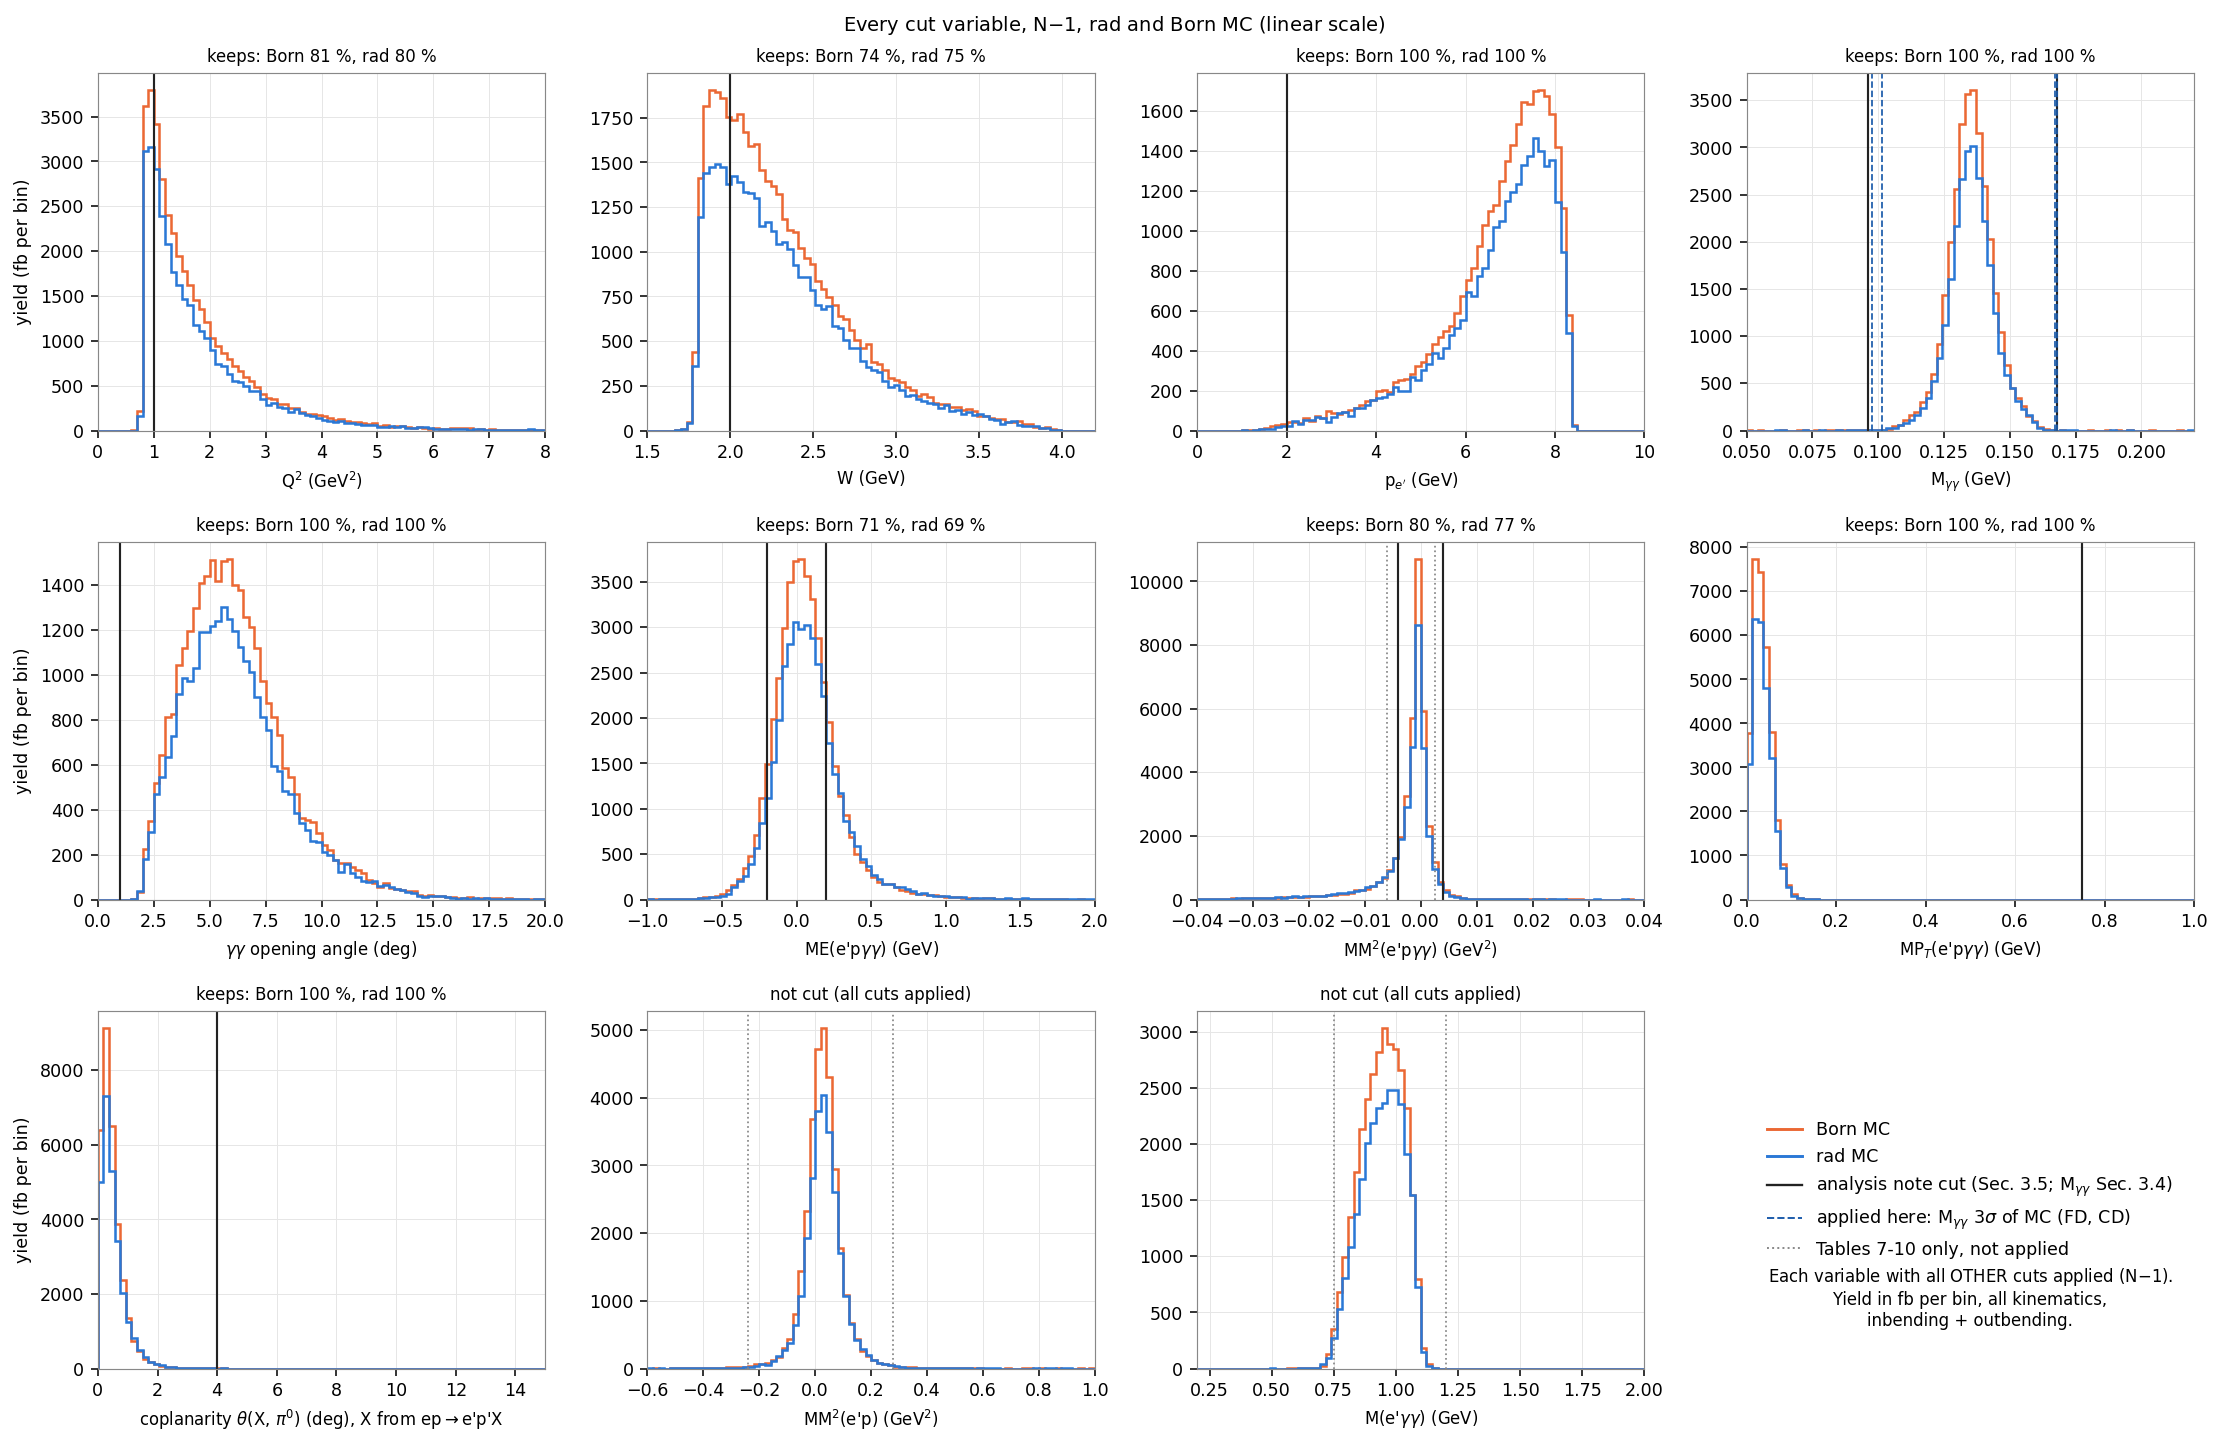
\includegraphics[width=\textwidth]{n1_cutvars_linear.png}
\caption{Every cut variable with all \emph{other} cuts applied (N$-$1), rad and Born MC, all
kinematics. Solid: the note's cut. Dotted: windows of Tables 7--10 that Sec.~3.5 does not list.}
\end{figure}

\begin{table}[H]\centering
\begin{tabular}{lcc}\toprule
cut, given all others & Born kept & rad kept\\\midrule
$Q^2>1$ & 81\% & 80\%\\
$W>2$ & 74\% & 75\%\\
$|ME|<0.2$ & \textbf{71\%} & \textbf{69\%}\\
$|\mmtot|<0.004$ & \textbf{80\%} & \textbf{77\%}\\
$p_{e'}$, $M_{\gamma\gamma}$, opening, $MP_T$, coplanarity & 100\% & 100\%\\\bottomrule
\end{tabular}
\caption{Only $ME$ and $\mmtot$ treat rad and Born differently.}
\end{table}

\begin{figure}[H]\centering
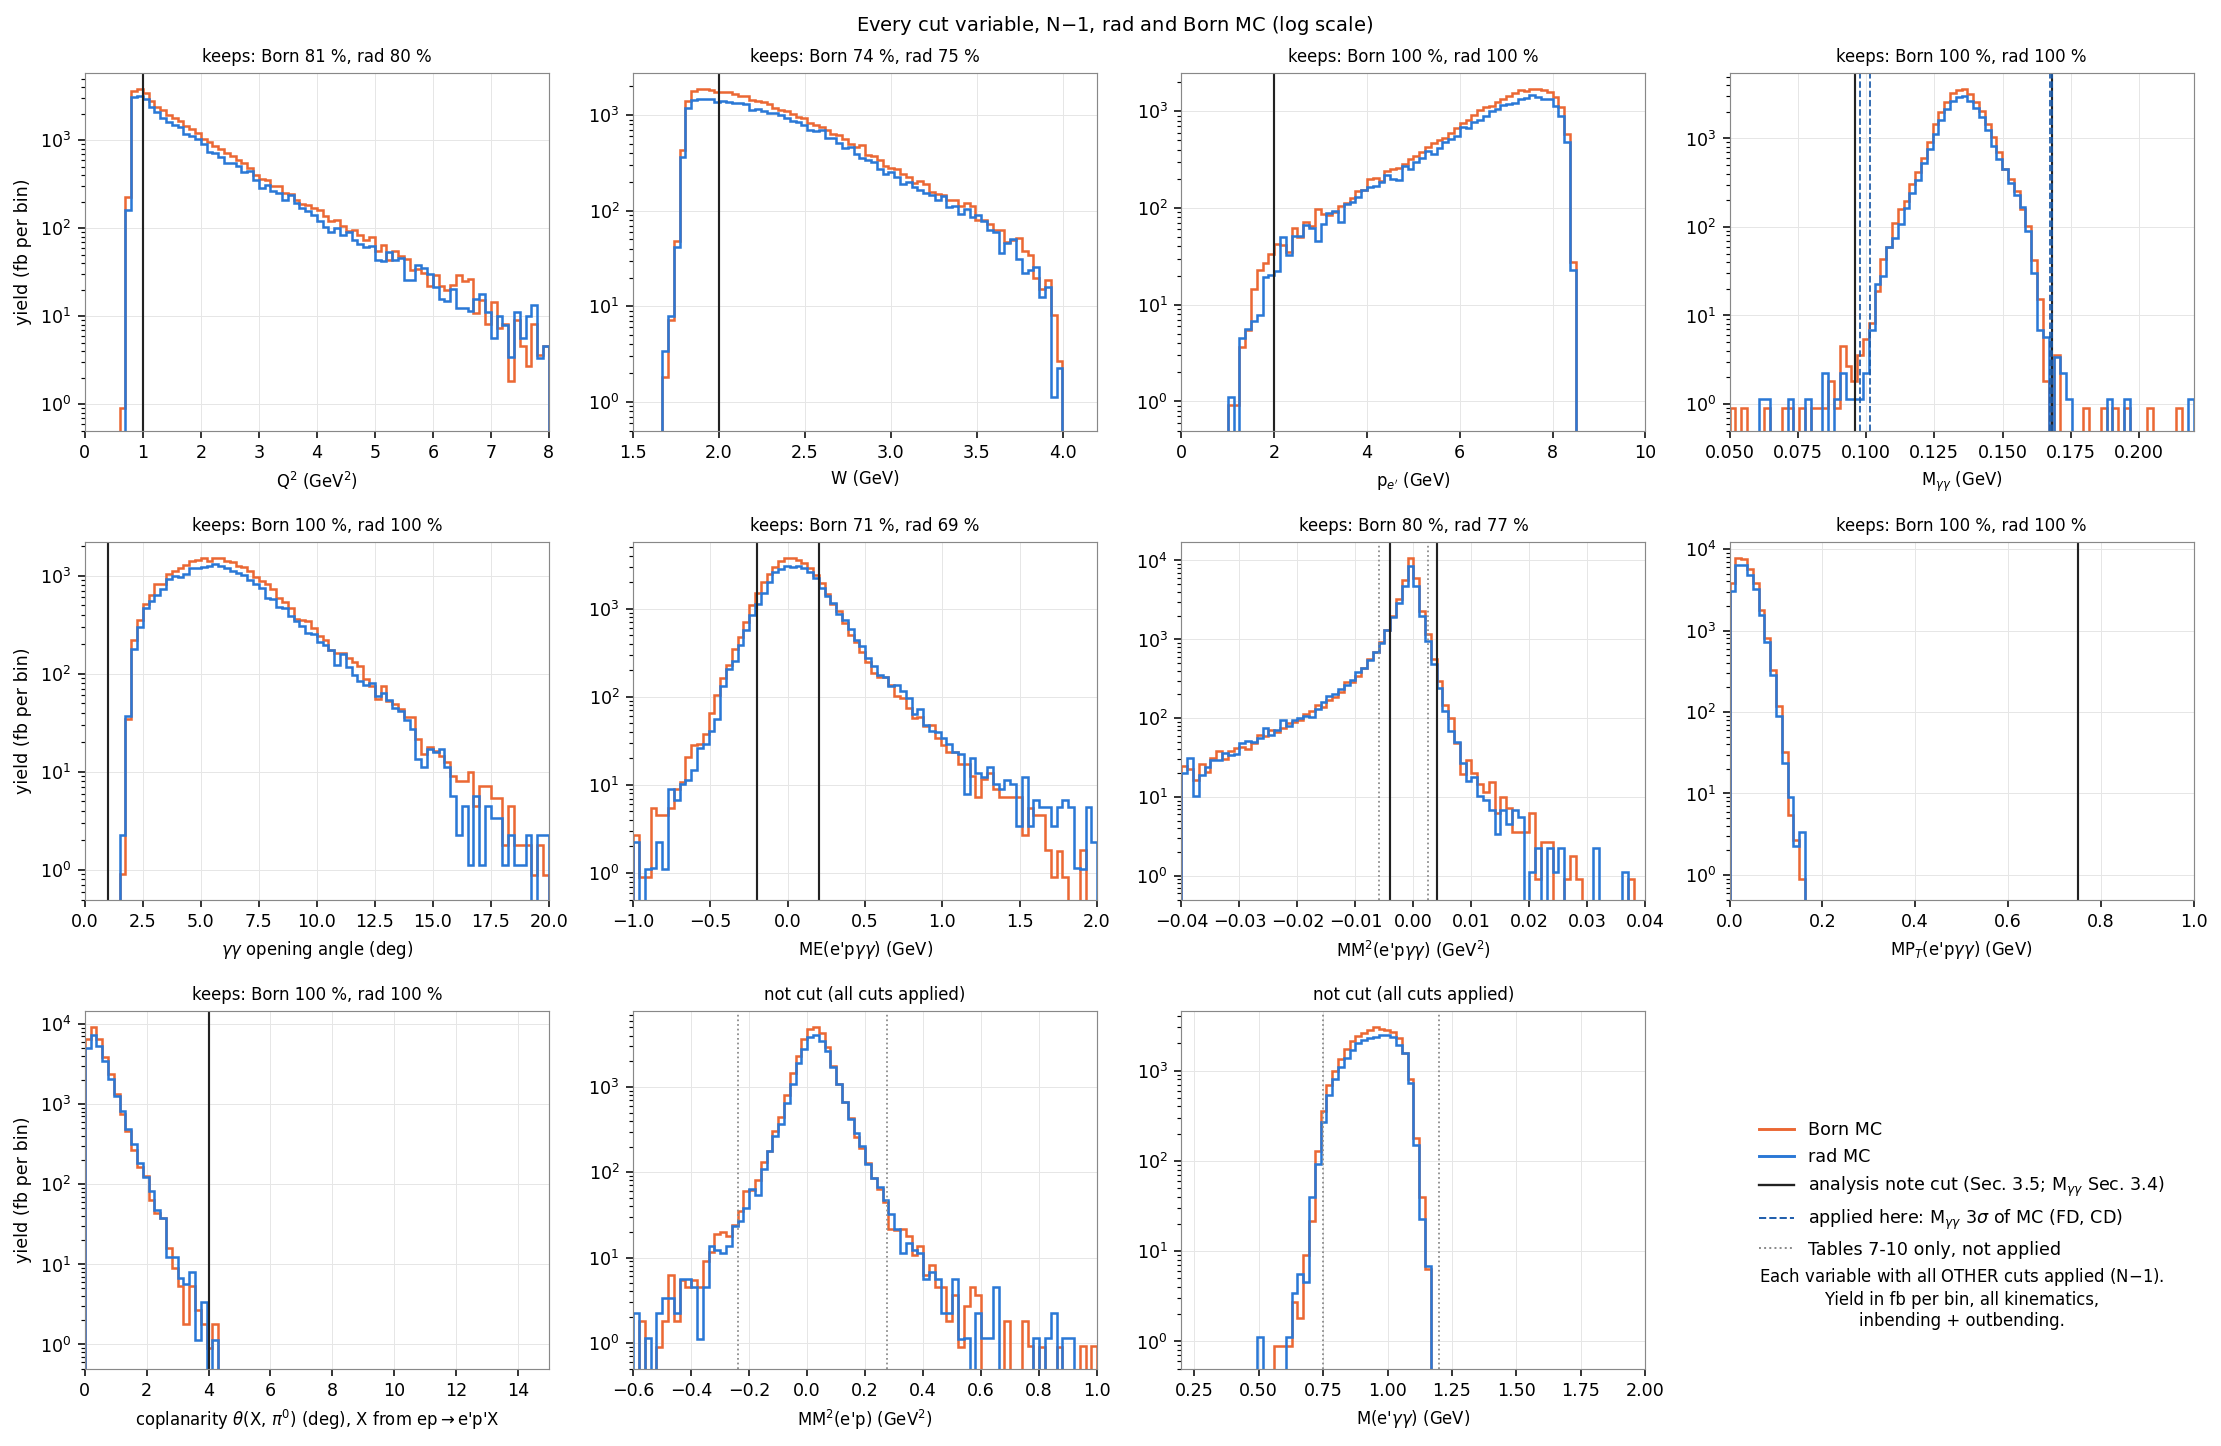
\includegraphics[width=\textwidth]{n1_cutvars_log.png}
\caption{As above, logarithmic scale.}
\end{figure}

%=====================================================================
\section{How the exclusivity cuts act on radiation}

For a radiative event with an unseen photon $k$:
\begin{align}
v&=\mmep-m_\pi^2=2p_\pi\!\cdot\!k=2E_kE_\pi(1-\beta_\pi\cos\theta_{\pi k}),\\
ME&=E_k,\qquad \mmtot=k^2=0,\qquad MP_T=k_T,\\
\tan\theta(X,\pi^0)&\approx\frac{E_k\sin\theta_{\pi k}}{E_\pi+E_k\cos\theta_{\pi k}} .
\end{align}
The missing-energy cut cuts the photon energy and maps onto $v$ through the photon's angle to the
$\pi^0$ (median $21^\circ$). $\mmtot$ vanishes for any real photon: it cuts radiation only through a
resolution that grows with $E_k$. The coplanarity angle grows like $\sin\theta_{\pi k}$ while $v$ grows
like $\theta_{\pi k}^2$, so it is the weaker cut.

\begin{figure}[H]\centering
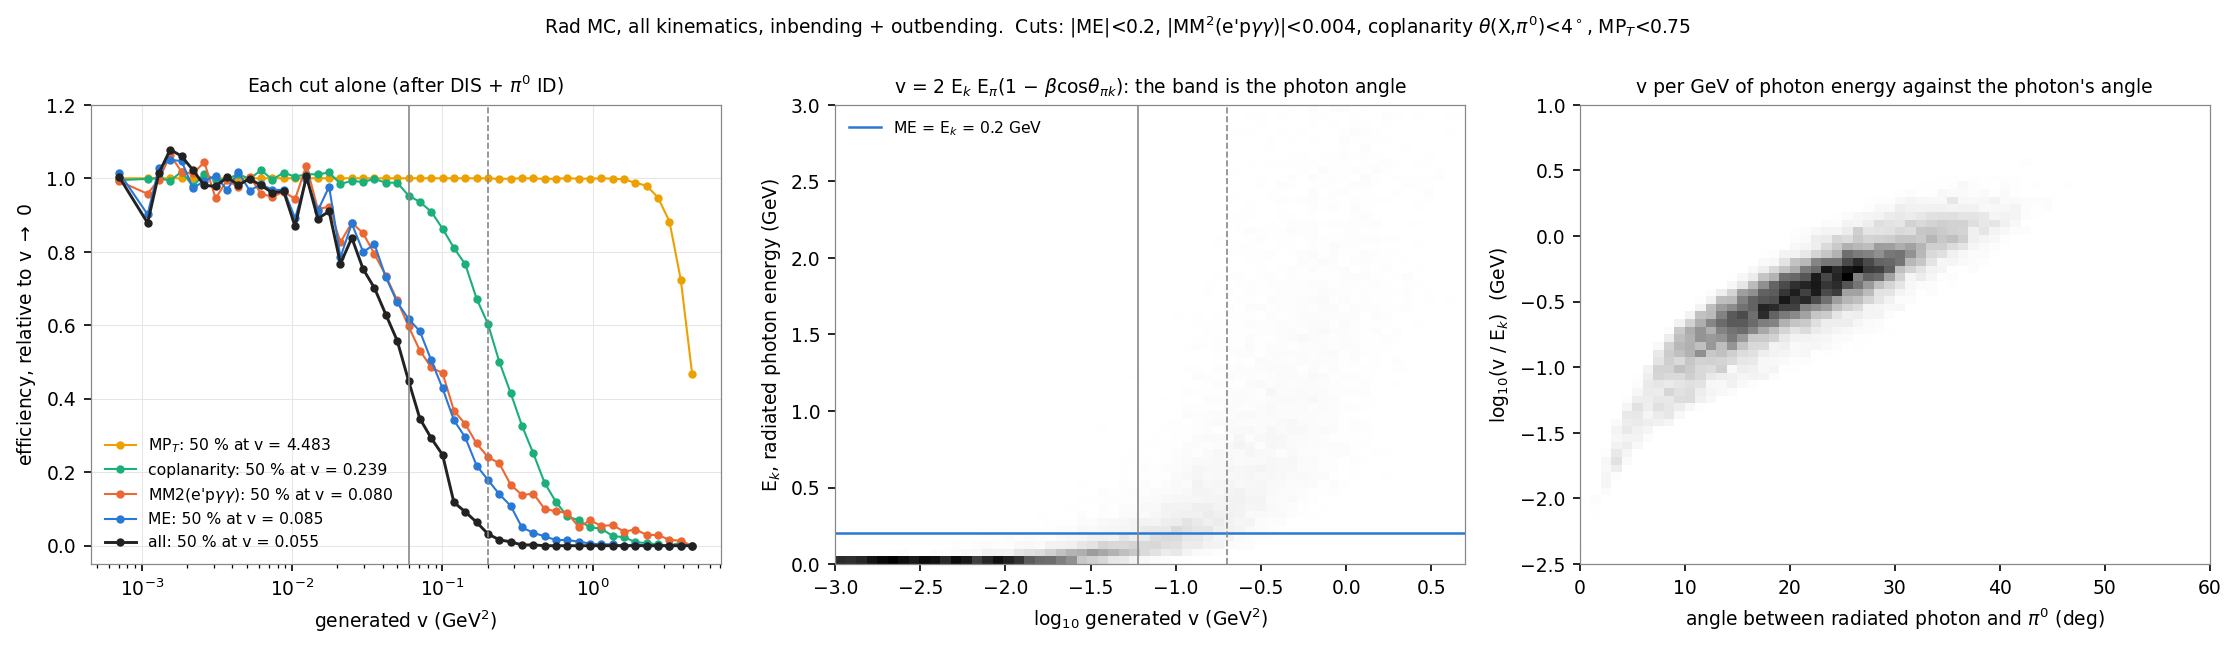
\includegraphics[width=\textwidth]{v3_each_cut.png}
\caption{Left: efficiency of each cut alone against the generated $v$; 50\% points
$ME$ 0.085, $\mmtot$ 0.080, coplanarity 0.24, $MP_T$ 4.5, all together 0.055~GeV$^2$.
Middle: photon energy against $v$. Right: $v/E_k$ against the photon--$\pi^0$ angle.}
\end{figure}

\begin{figure}[H]\centering
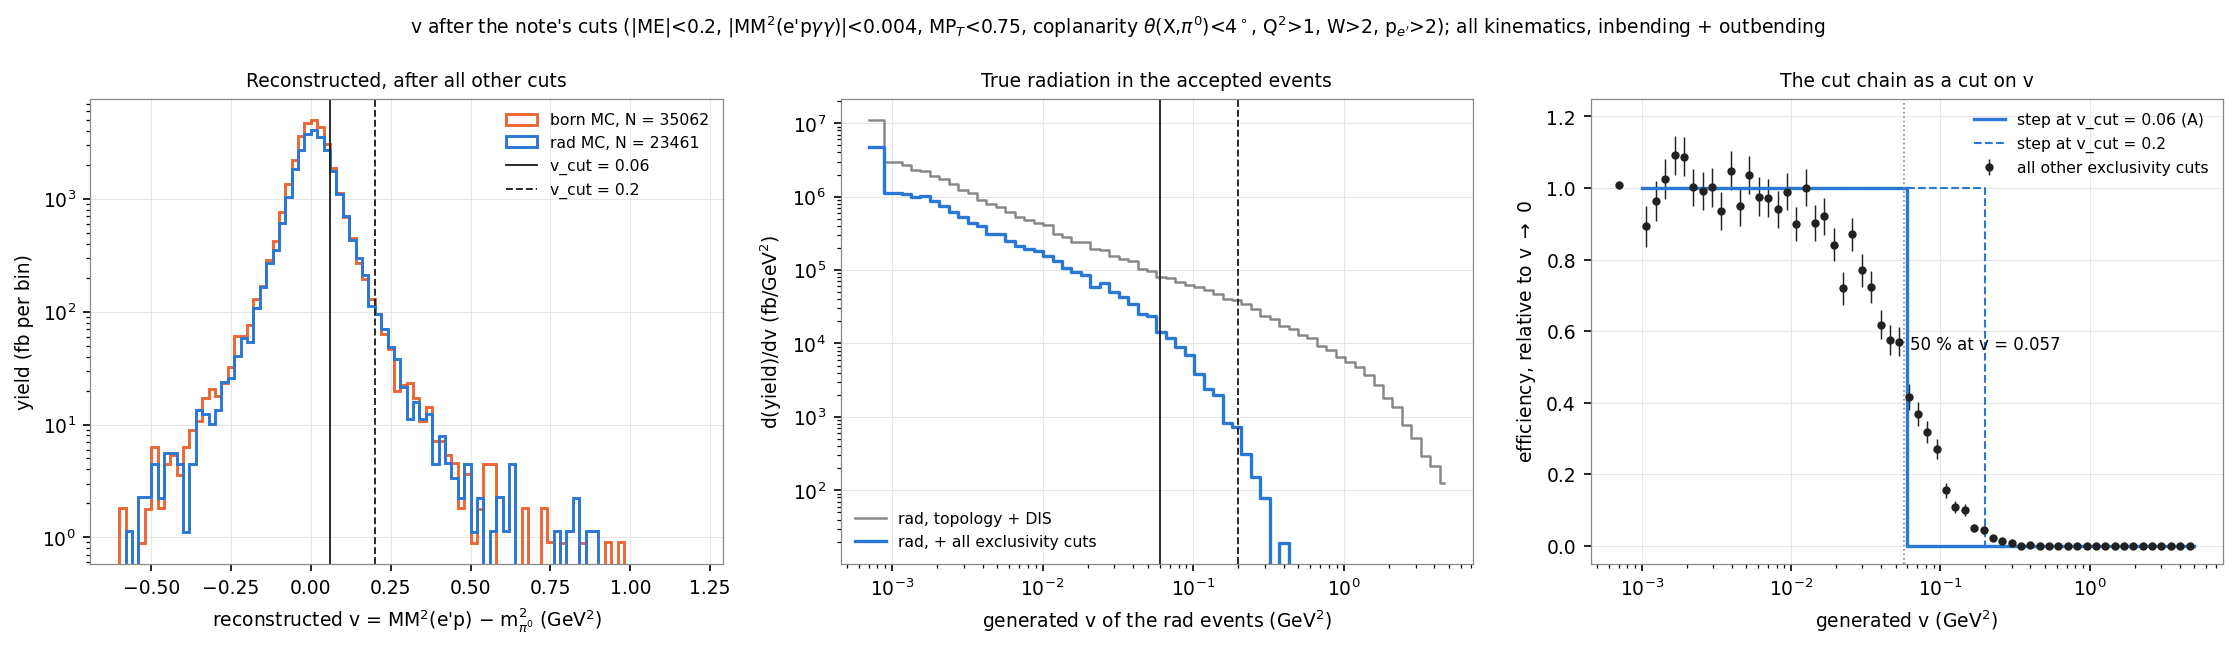
\includegraphics[width=\textwidth]{v1_vdist.png}
\caption{$v$ after all other cuts. Left: reconstructed. Middle: generated $v$ of the accepted rad
events before and after the exclusivity cuts. Right: the cut chain as an efficiency in $v$: flat to
$v\approx0.01$, 50\% at $v=0.057$, near zero above 0.2. Only 2.0\% of the accepted rad yield has
$v>0.066$, 0.09\% has $v>0.2$.}
\end{figure}

\begin{figure}[H]\centering
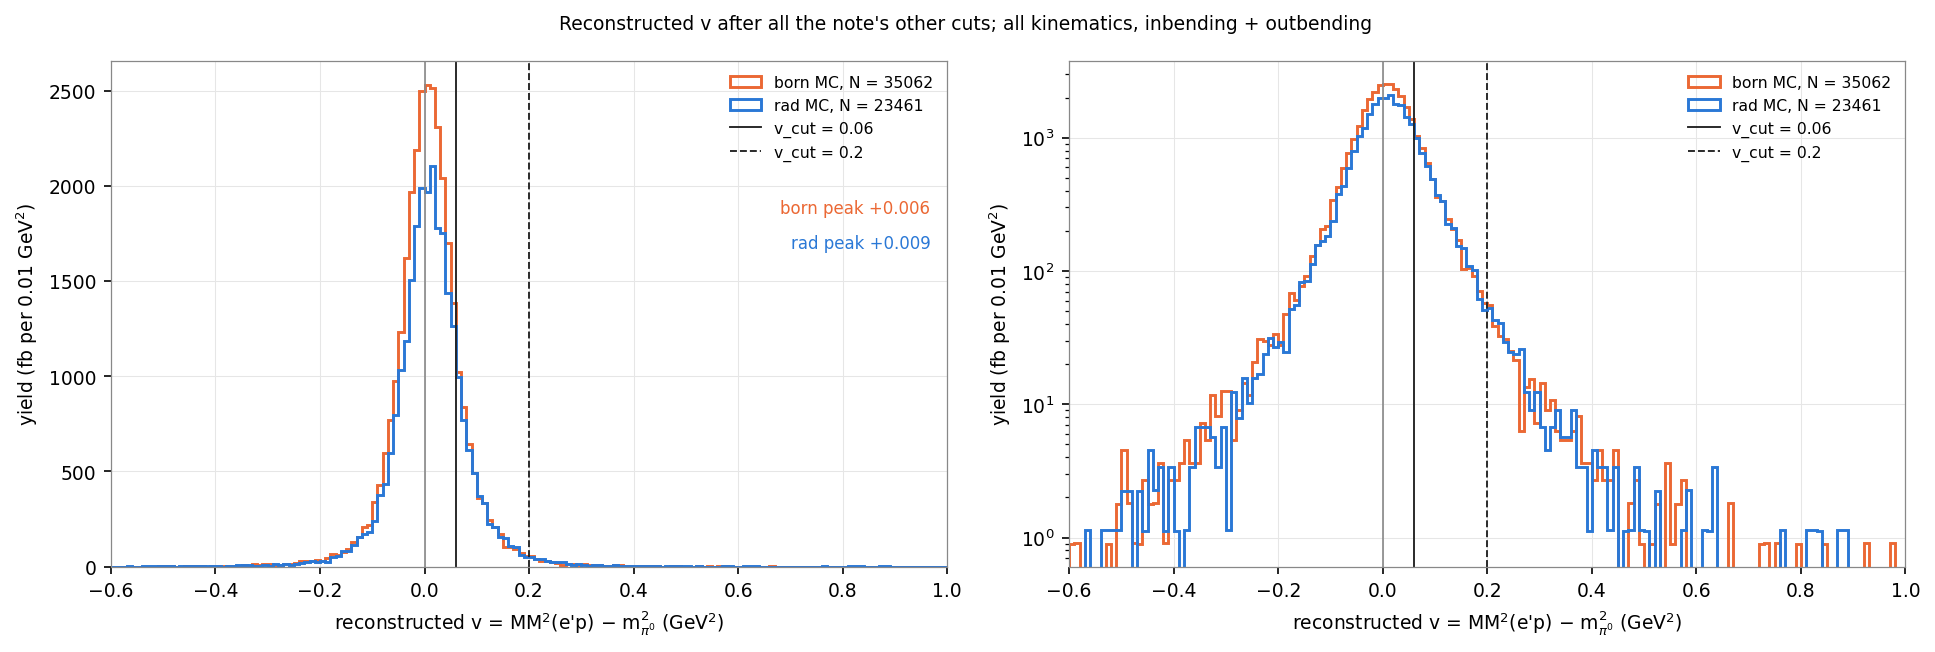
\includegraphics[width=\textwidth]{v2_vrec_lin_log.png}
\caption{Reconstructed $v$ after all other cuts, linear and log. The peak is at $+0.006$ (Born) and
$+0.009$~GeV$^2$ (rad): reconstructed momenta are 0.6\% (proton) and 0.1\% (electron) low, no
energy-loss correction. The core half-width is $\approx0.04$~GeV$^2$; the reconstructed $\mmep$
cannot resolve a $\vcut$ of 0.06.}
\end{figure}

%=====================================================================
\section{One wide bin, $\phi$ by $\phi$ (MC-calibrated windows)}

First pass, $1.5<Q^2<2.5$, $0.15<x_B<0.30$, $0.2<-t<0.6$, with each exclusivity window set to
$\pm3\sigma$ of the Born MC (not the note's literal values).

\begin{figure}[H]\centering
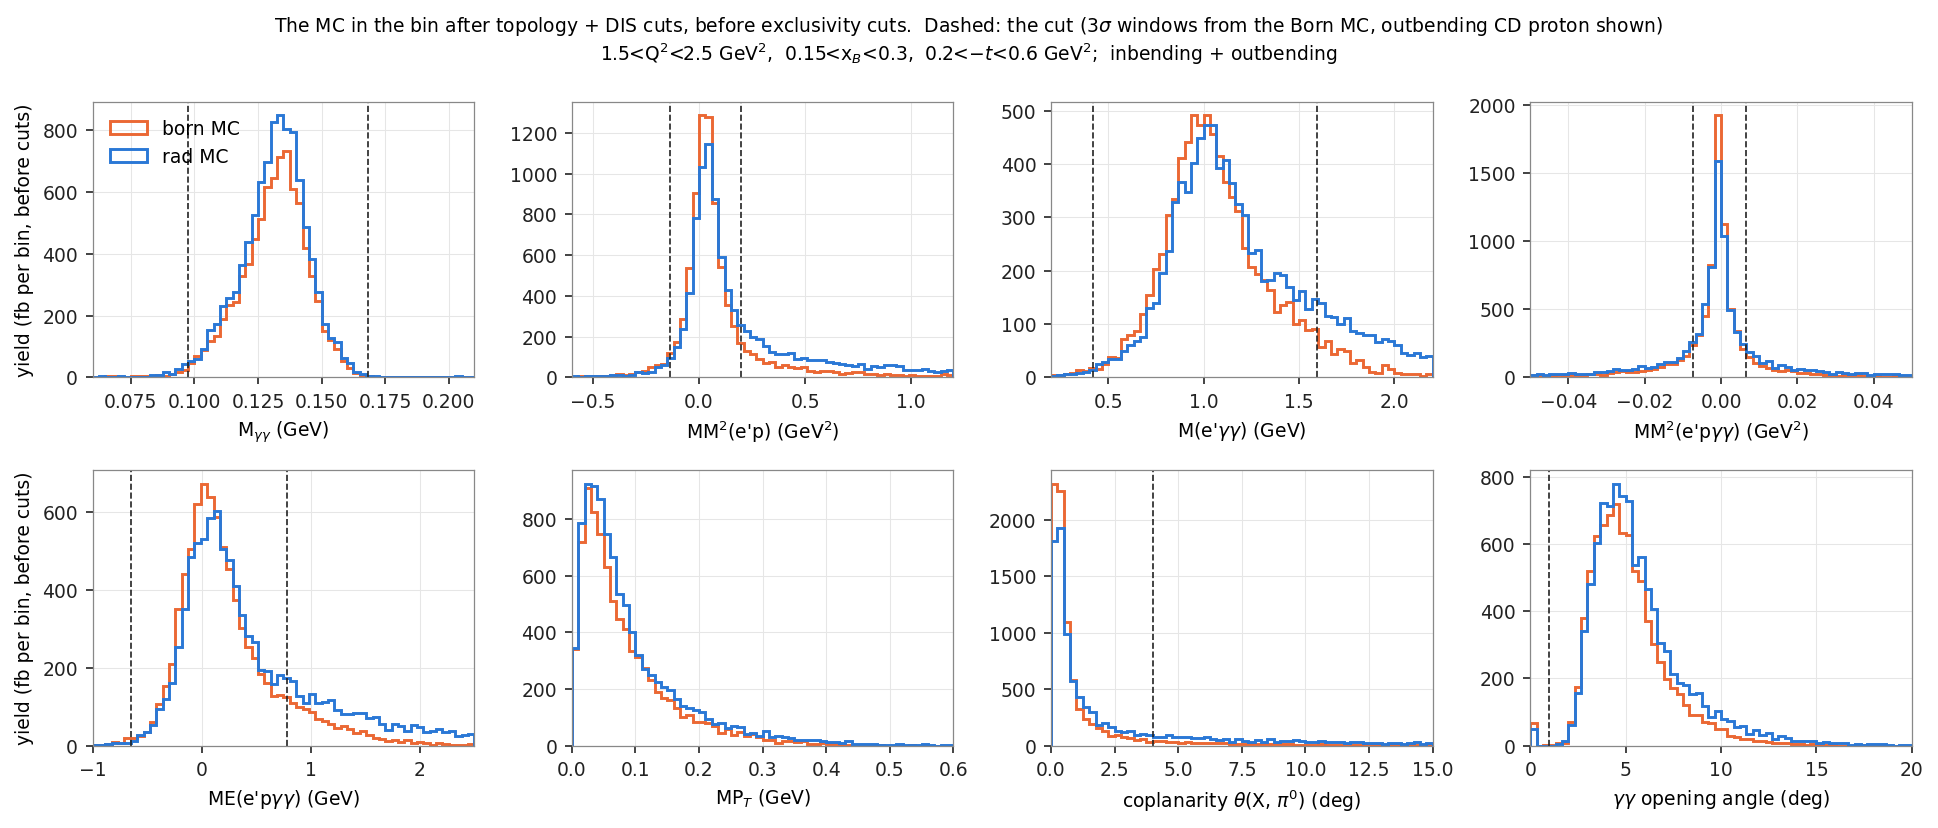
\includegraphics[width=\textwidth]{p1_exclusivity.png}
\caption{The MC in the bin before exclusivity cuts.}
\end{figure}
\begin{figure}[H]\centering
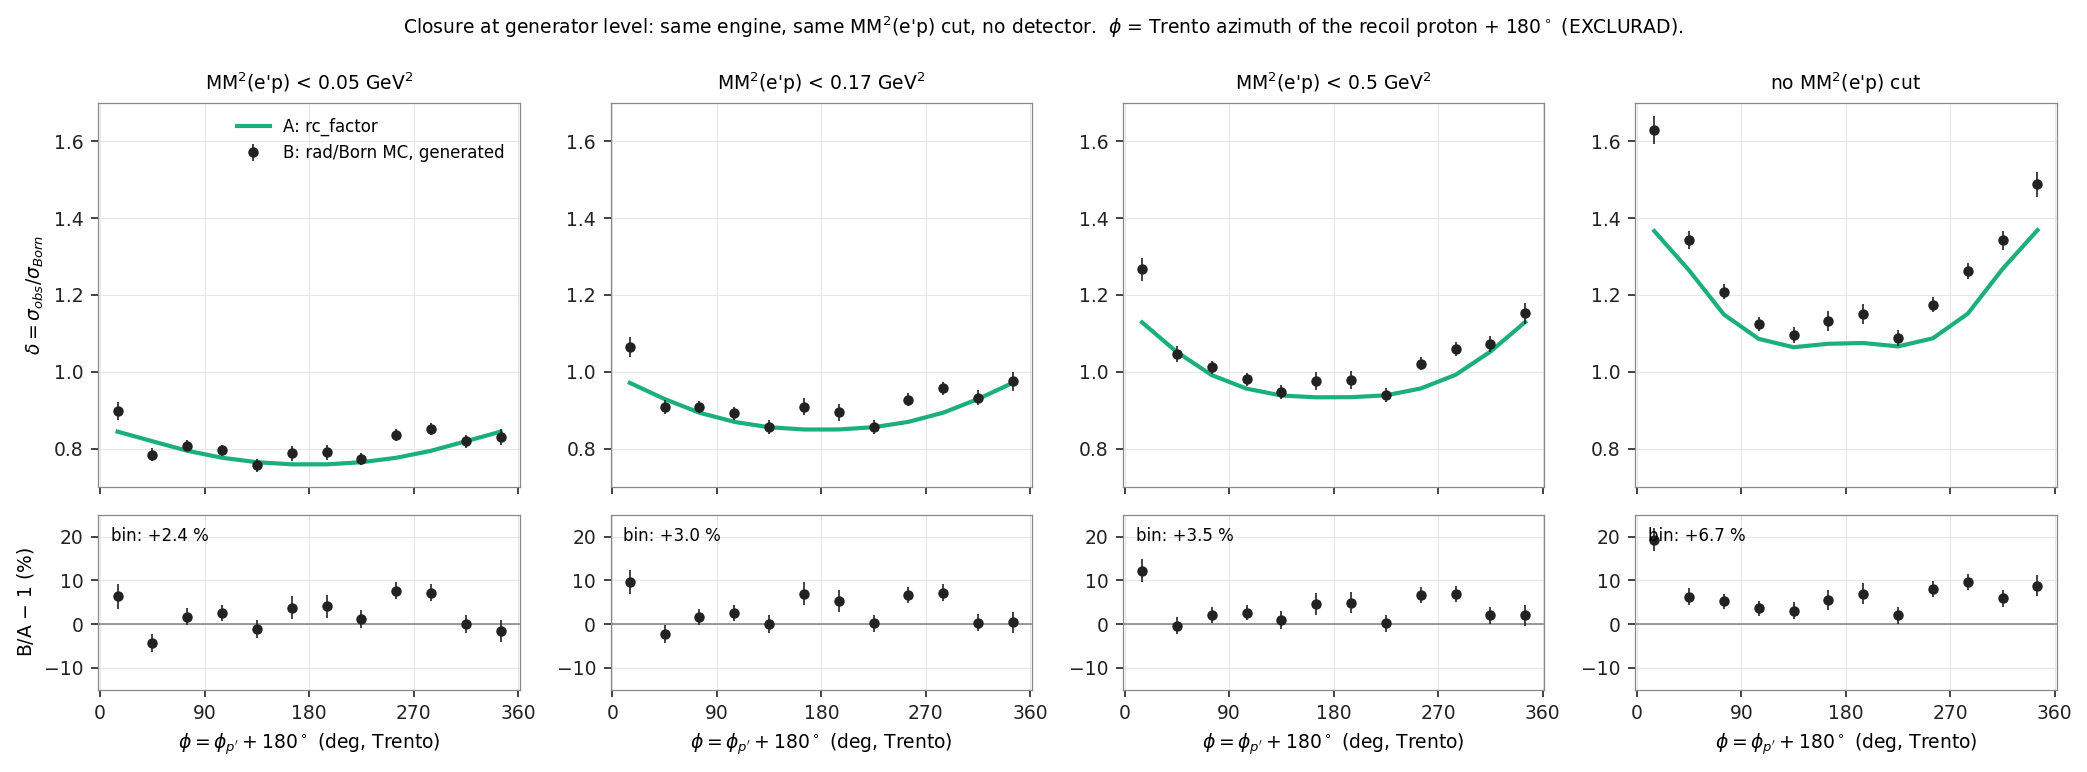
\includegraphics[width=\textwidth]{p3_closure.png}
\caption{Closure at generator level: same engine, same $\mmep$ cut, no detector. B follows A in shape
at every cut; the bin-integrated $+3\%$ is \texttt{itarg} in the Born arm.}
\end{figure}
\begin{figure}[H]\centering
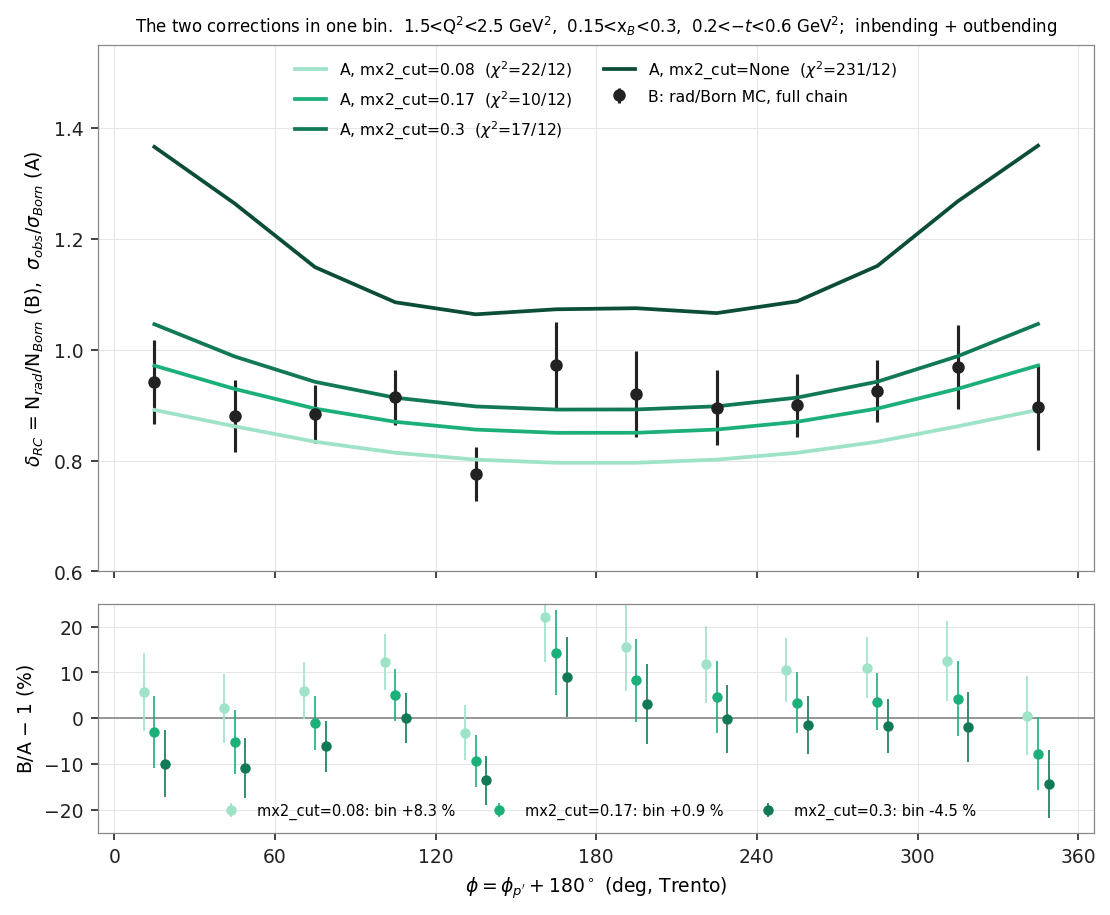
\includegraphics[width=0.75\textwidth]{p4_A_vs_B.png}
\caption{$\delta_B(\phi)$ with the full chain against $\delta_A(\phi)$ for several $\vcut$;
B/A$-1$ in \% below. Best $\vcut=0.17$, $\chi^2=9.7/12$; errors 5--8\% per $\phi$ bin.}
\end{figure}
\begin{figure}[H]\centering
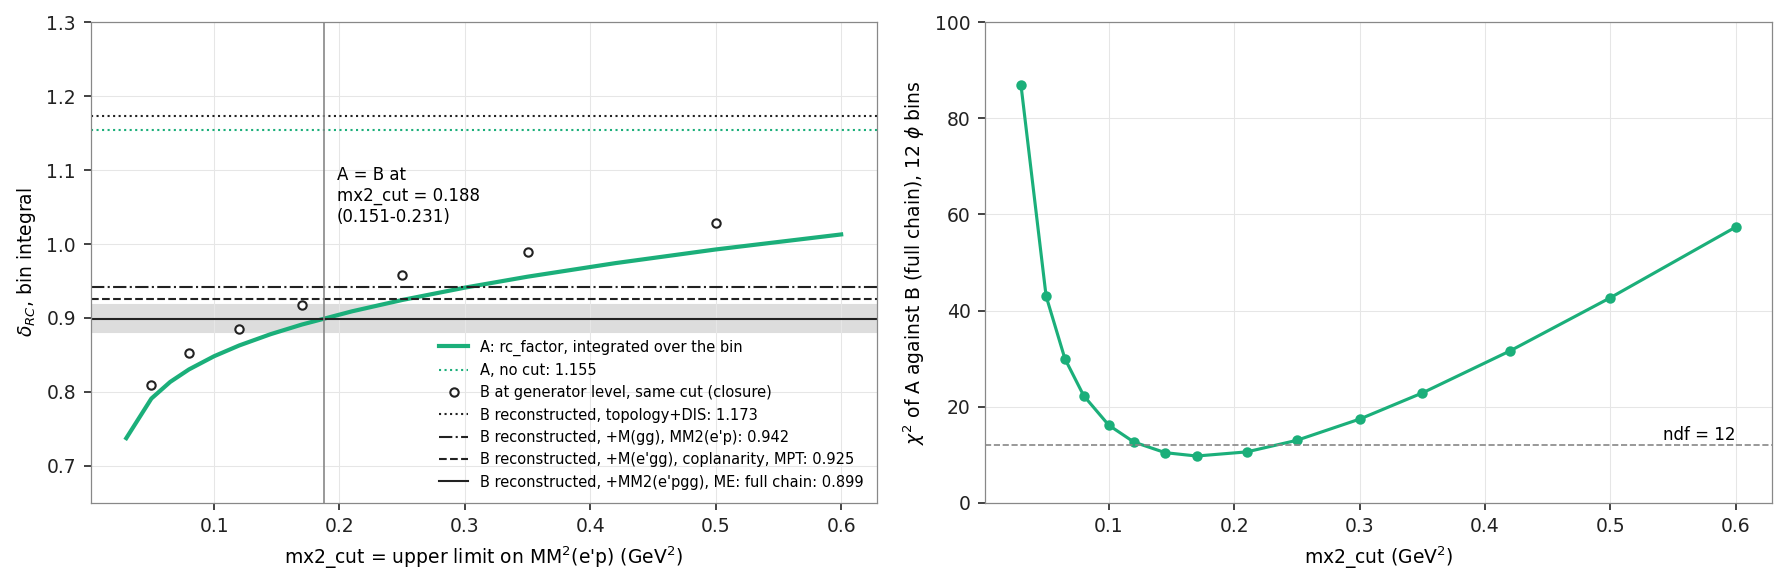
\includegraphics[width=\textwidth]{p5_scan.png}
\caption{Bin integral against $\vcut$ and $\chi^2$ of A against B.}
\end{figure}
\begin{figure}[H]\centering
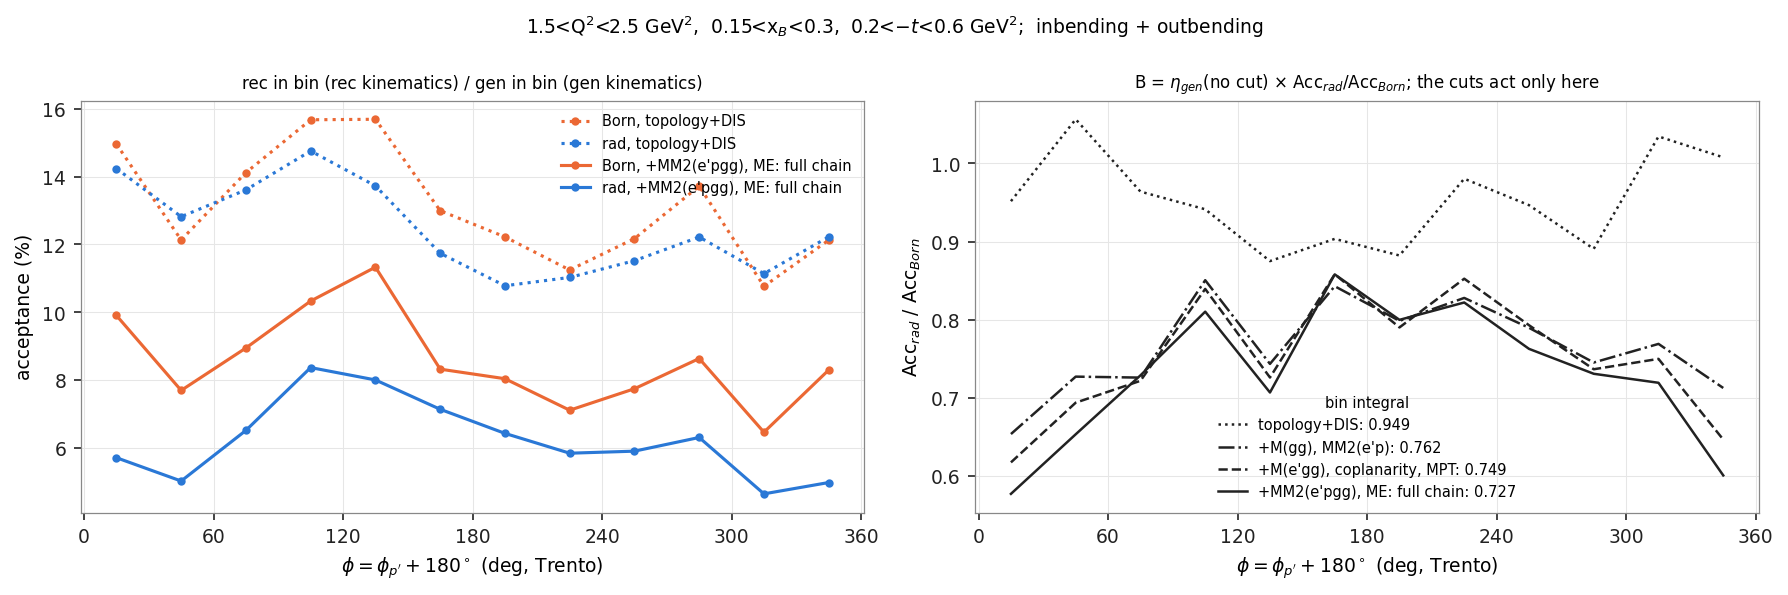
\includegraphics[width=\textwidth]{p6_acceptance.png}
\caption{The two acceptances and their ratio: the cuts act on $\delta_B$ only through
Acc$_{\rm rad}$/Acc$_{\rm Born}$ (0.95 after topology+DIS, 0.73 after the full chain).}
\end{figure}

%=====================================================================
\section{The note's grid, MC-calibrated windows}

\begin{figure}[H]\centering
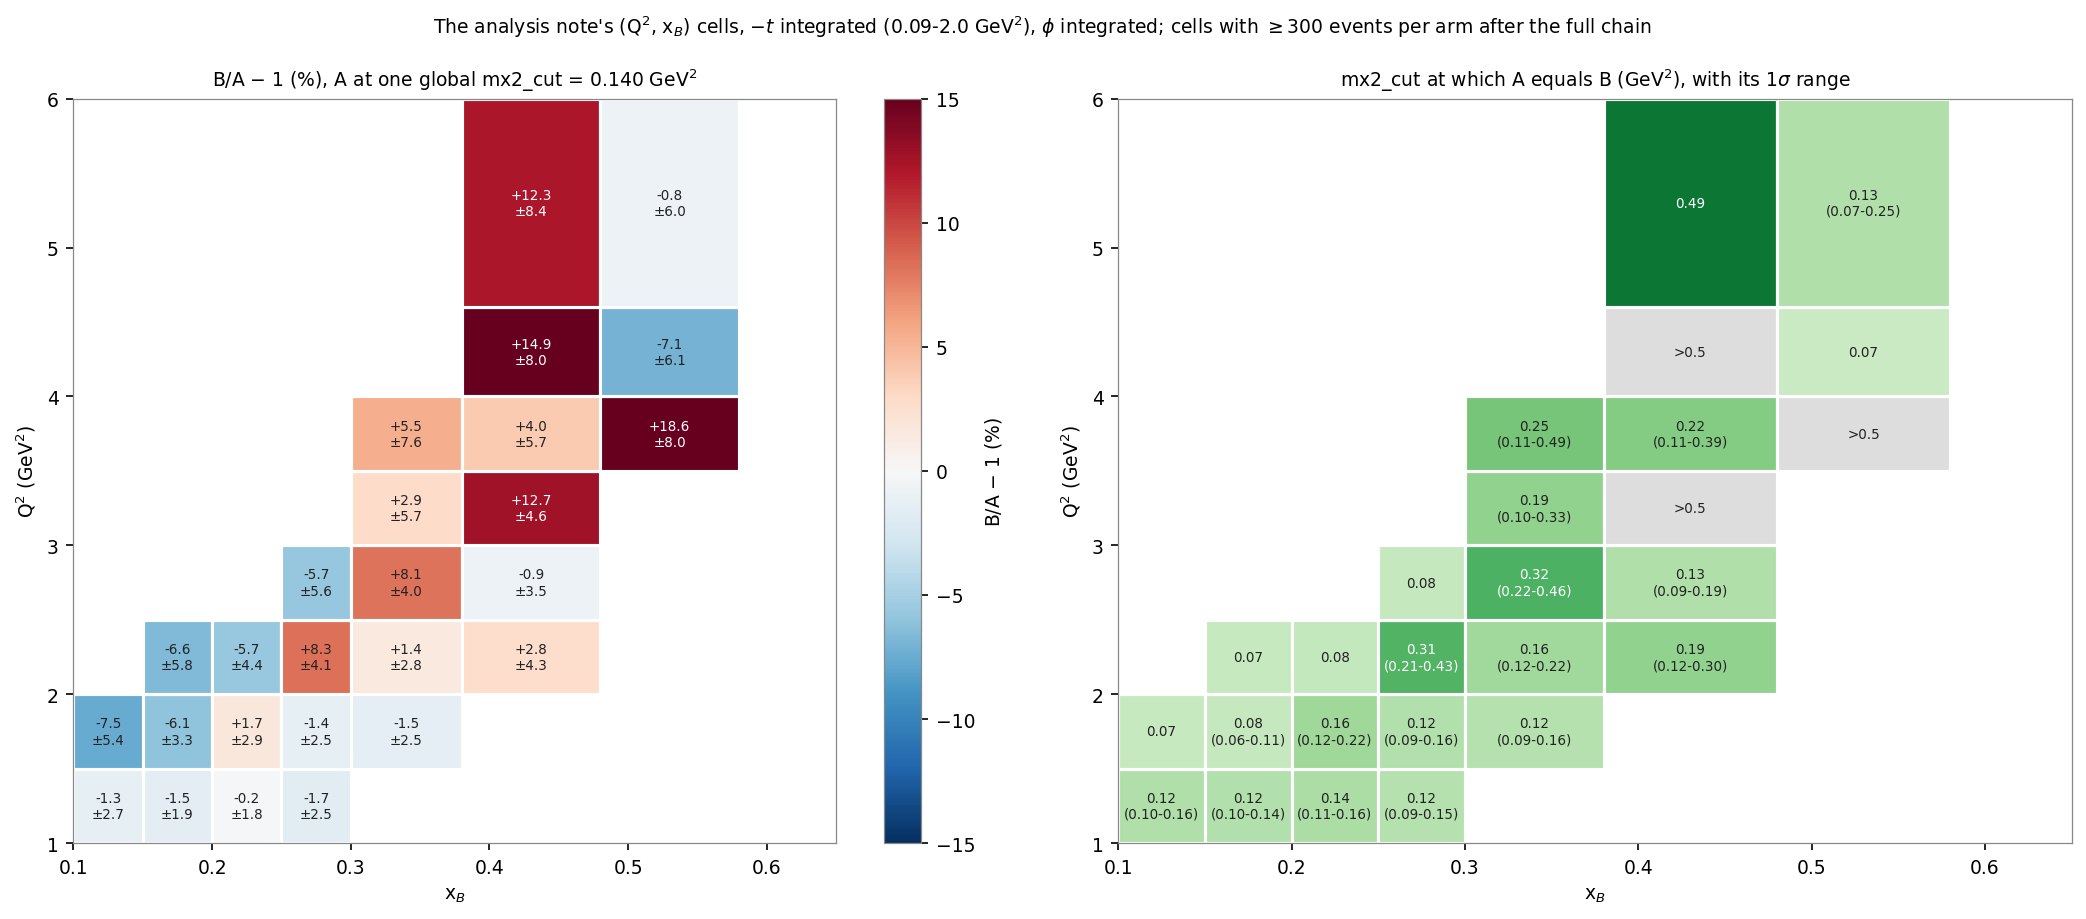
\includegraphics[width=\textwidth]{g1_map.png}
\caption{$(Q^2,x_B)$ cells, $-t$ and $\phi$ integrated. Left: B/A$-1$ at the best global
$\vcut=0.14$ ($\chi^2=42/26$). Right: the $\vcut$ at which A equals B, cell by cell.}
\end{figure}
\begin{figure}[H]\centering
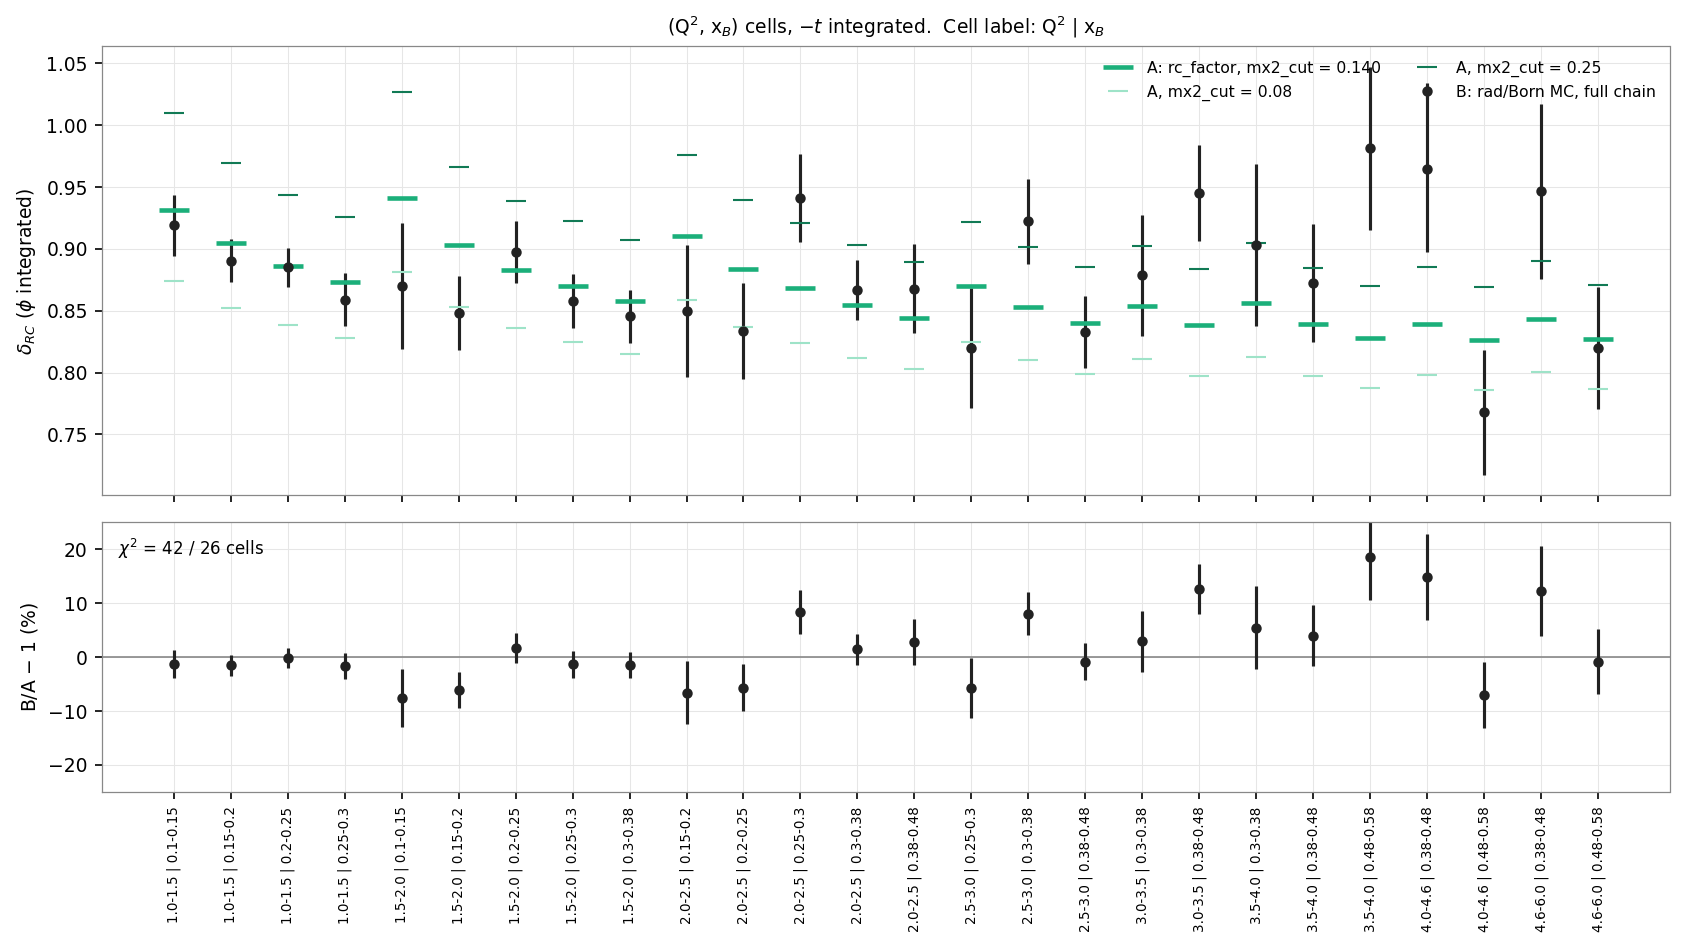
\includegraphics[width=\textwidth]{g2_cells_2d.png}
\caption{B and A per $(Q^2,x_B)$ cell, B/A$-1$ in \% below. With these wider windows the high
$Q^2$/$x_B$ cells are 10--18\% off.}
\end{figure}
\begin{figure}[H]\centering
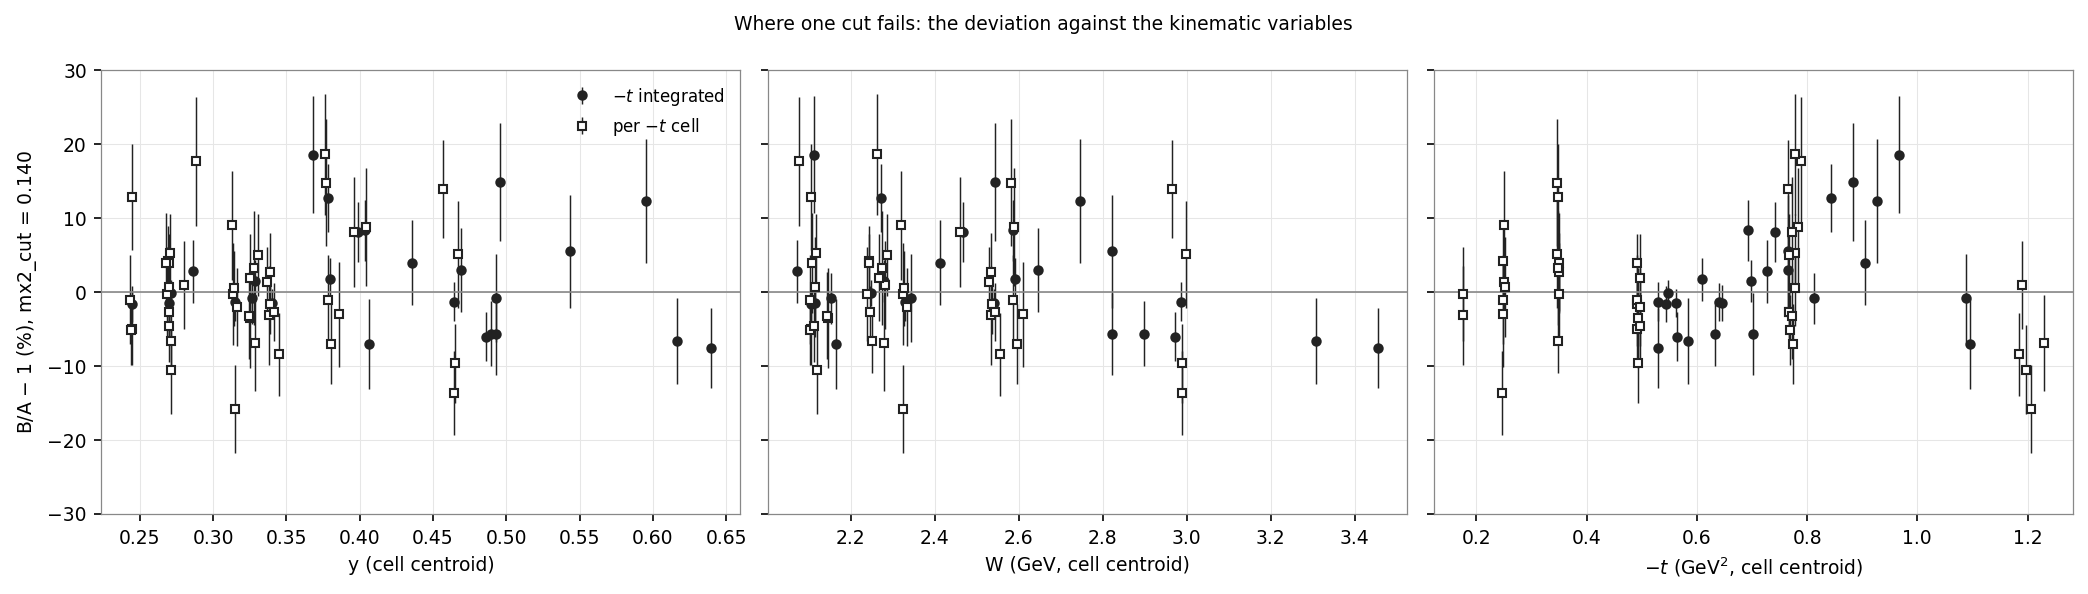
\includegraphics[width=\textwidth]{g3_vs_kin.png}
\caption{Deviation against $y$, $W$ and $-t$ of the cell centroid.}
\end{figure}

%=====================================================================
\section{The note's cuts as printed: every combination of $Q^2$, $x_B$, $-t$}

\begin{figure}[H]\centering
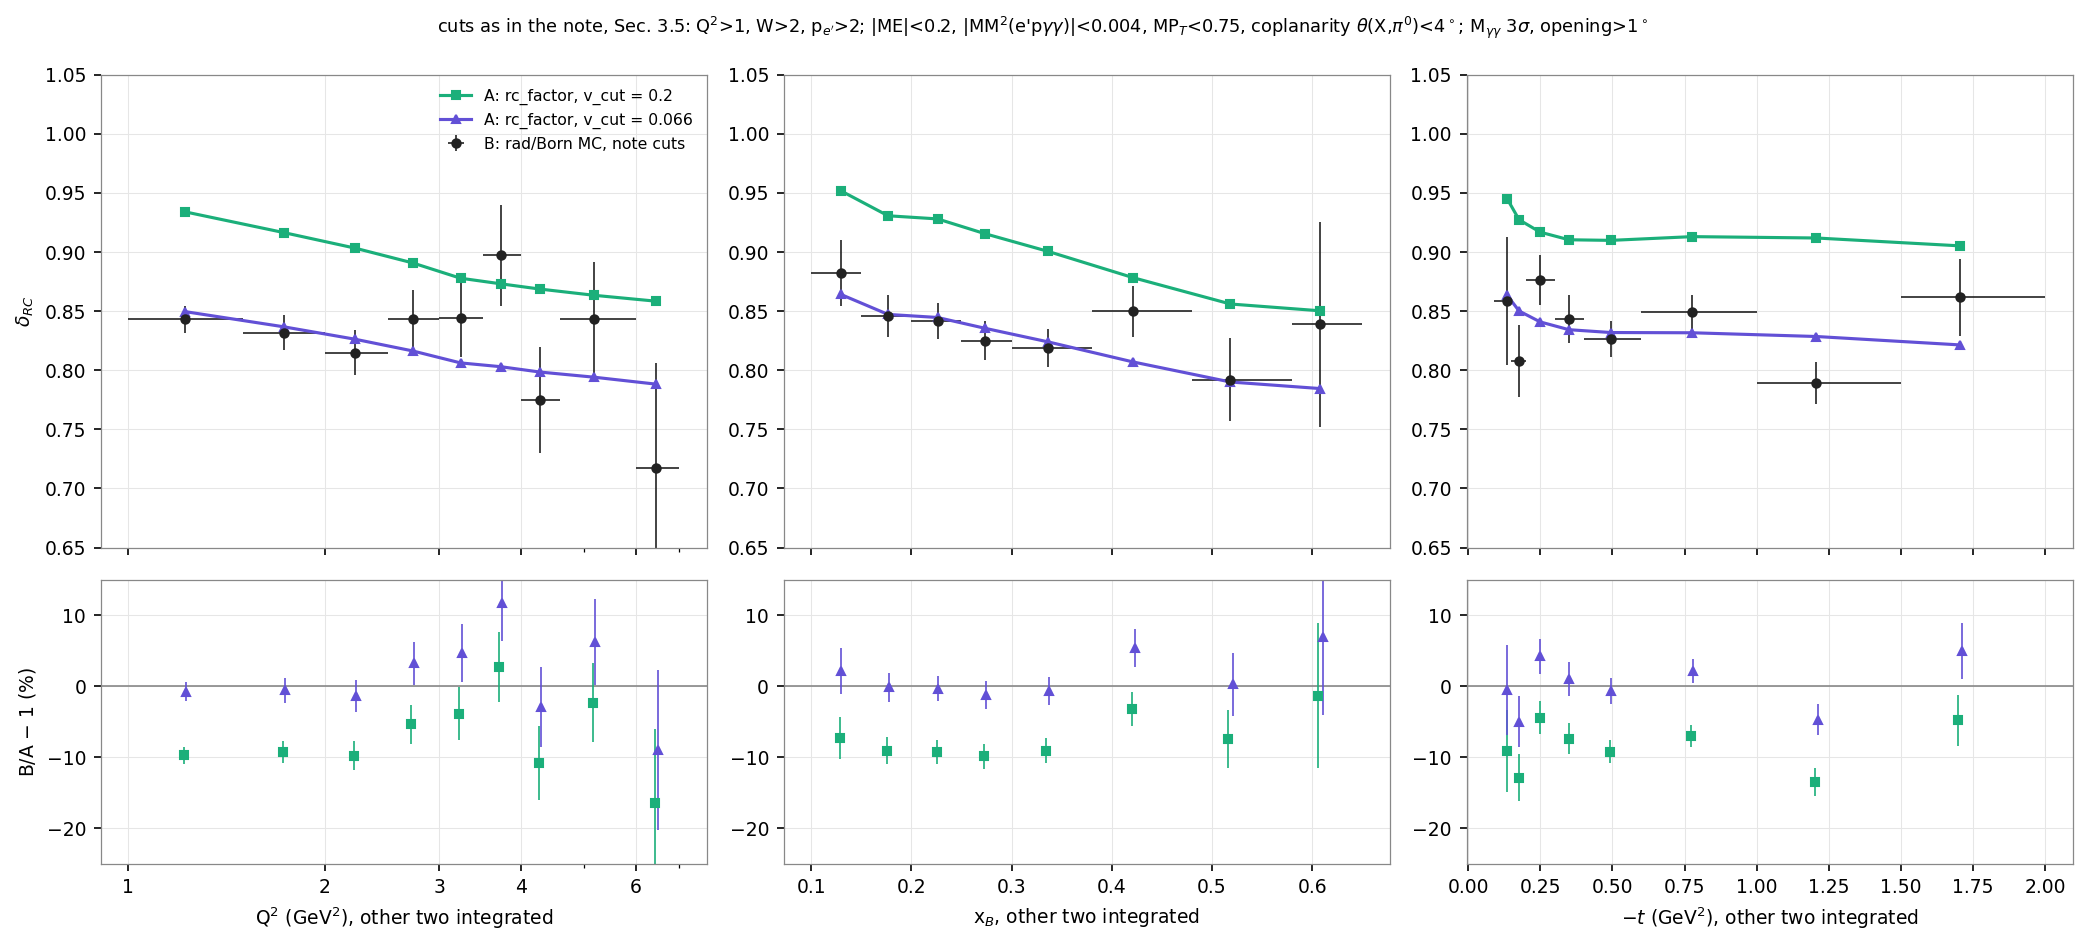
\includegraphics[width=\textwidth]{c1_one_variable.png}
\caption{One variable at a time, the other two integrated. A at $\vcut=0.2$ (green) is 5--10\% above
B; A at the best global $\vcut=0.066$ (violet) agrees.}
\end{figure}
\begin{figure}[H]\centering
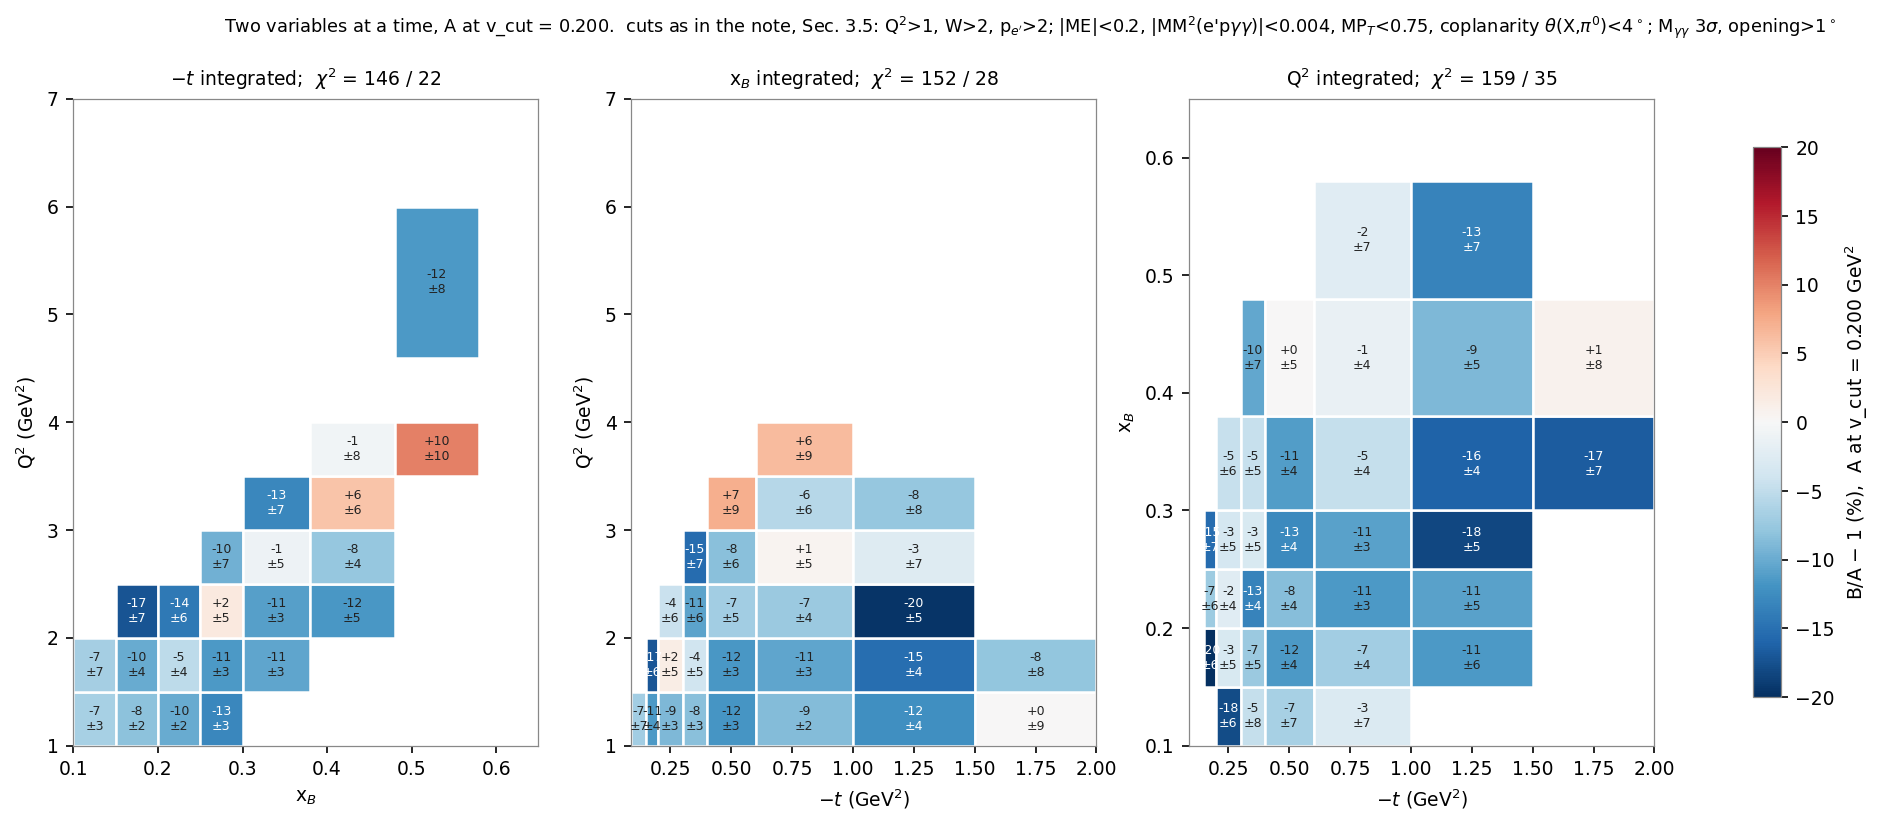
\includegraphics[width=\textwidth]{c2_maps_v0.png}
\caption{Two variables at a time, A at $\vcut=0.2$. Cell text: B/A$-1$ (\%) $\pm$ error.}
\end{figure}
\begin{figure}[H]\centering
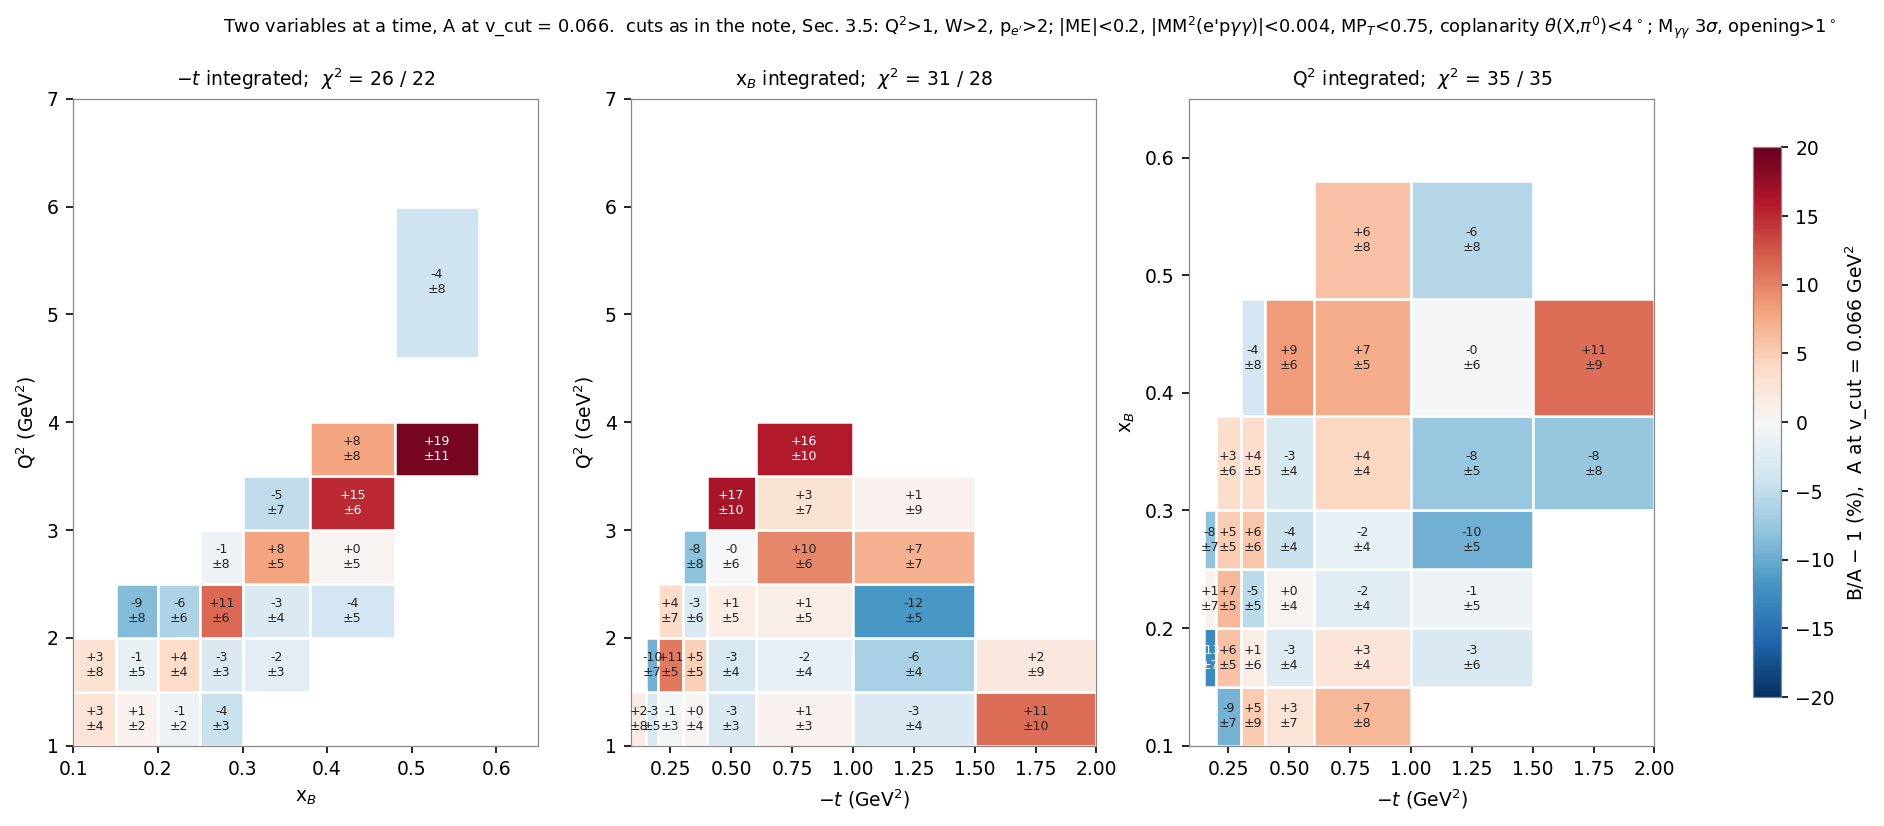
\includegraphics[width=\textwidth]{c2_maps_vbest.png}
\caption{Two variables at a time, A at $\vcut=0.066$.}
\end{figure}
\begin{figure}[H]\centering
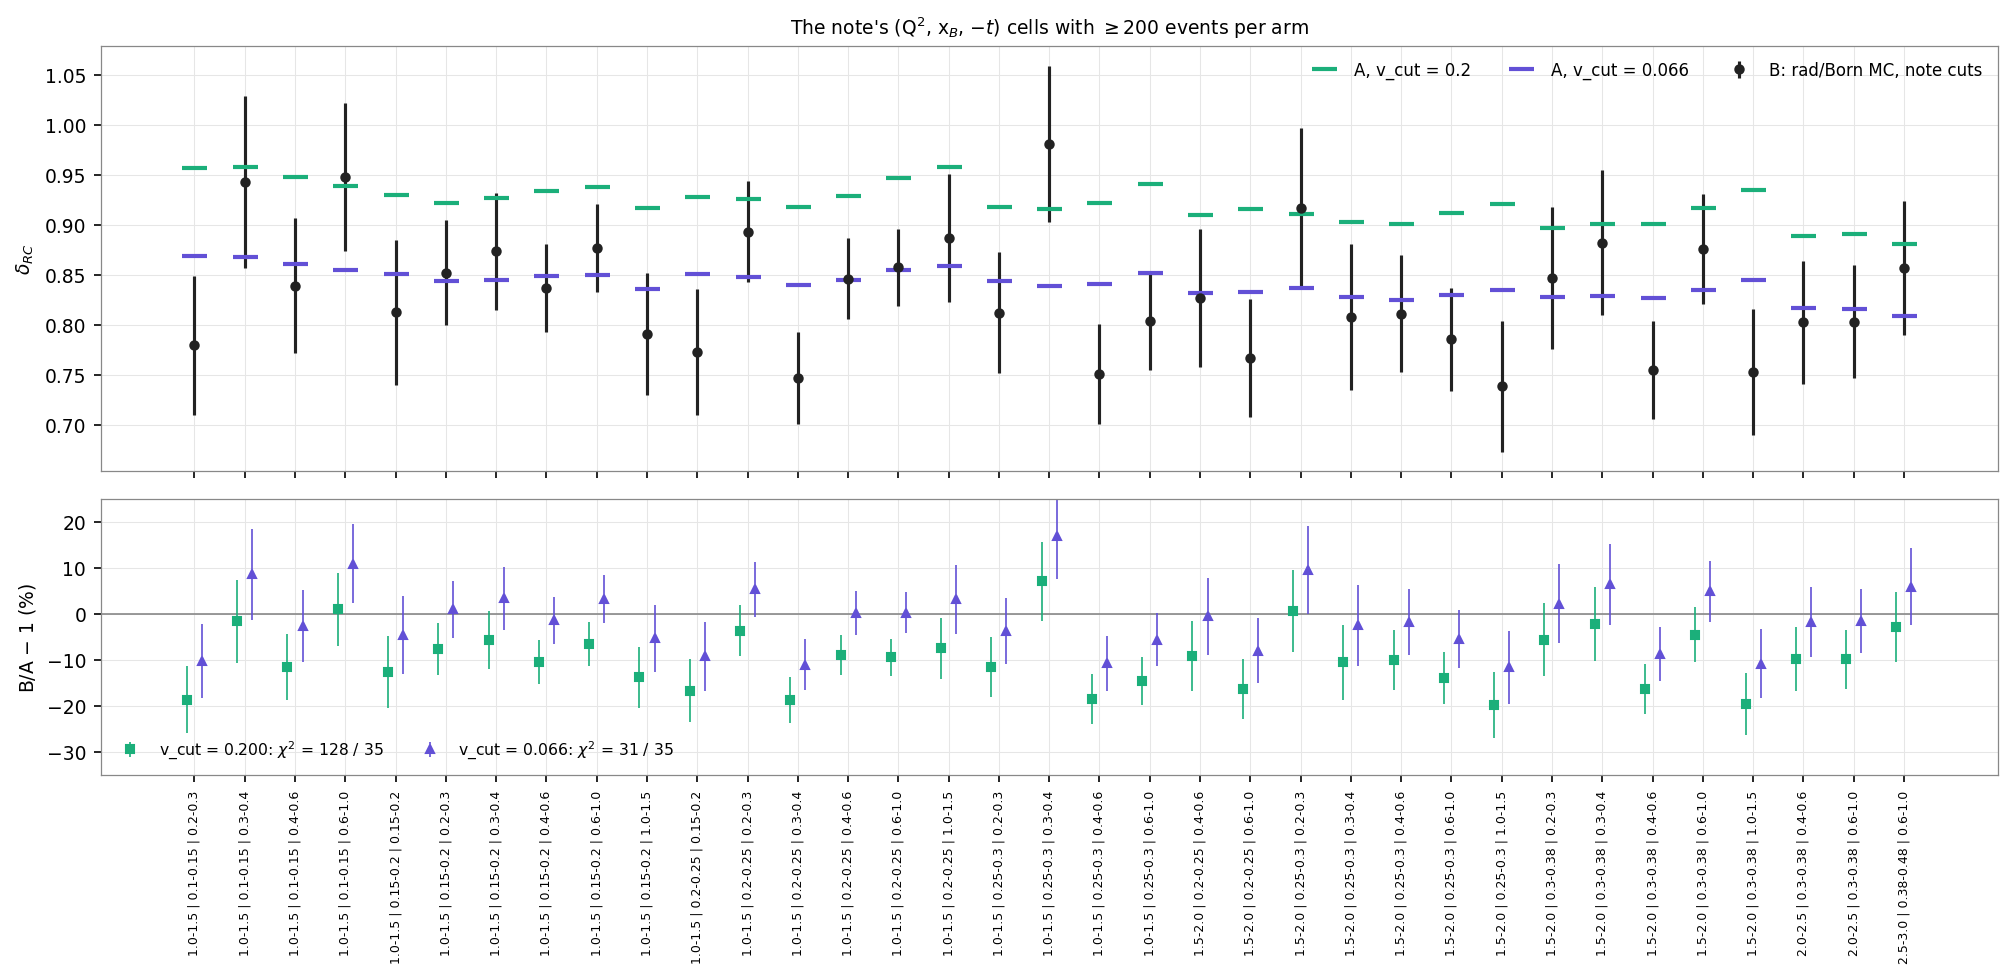
\includegraphics[width=\textwidth]{c3_cells_3d.png}
\caption{All three variables, cells with $\ge200$ events per arm.}
\end{figure}
\begin{figure}[H]\centering
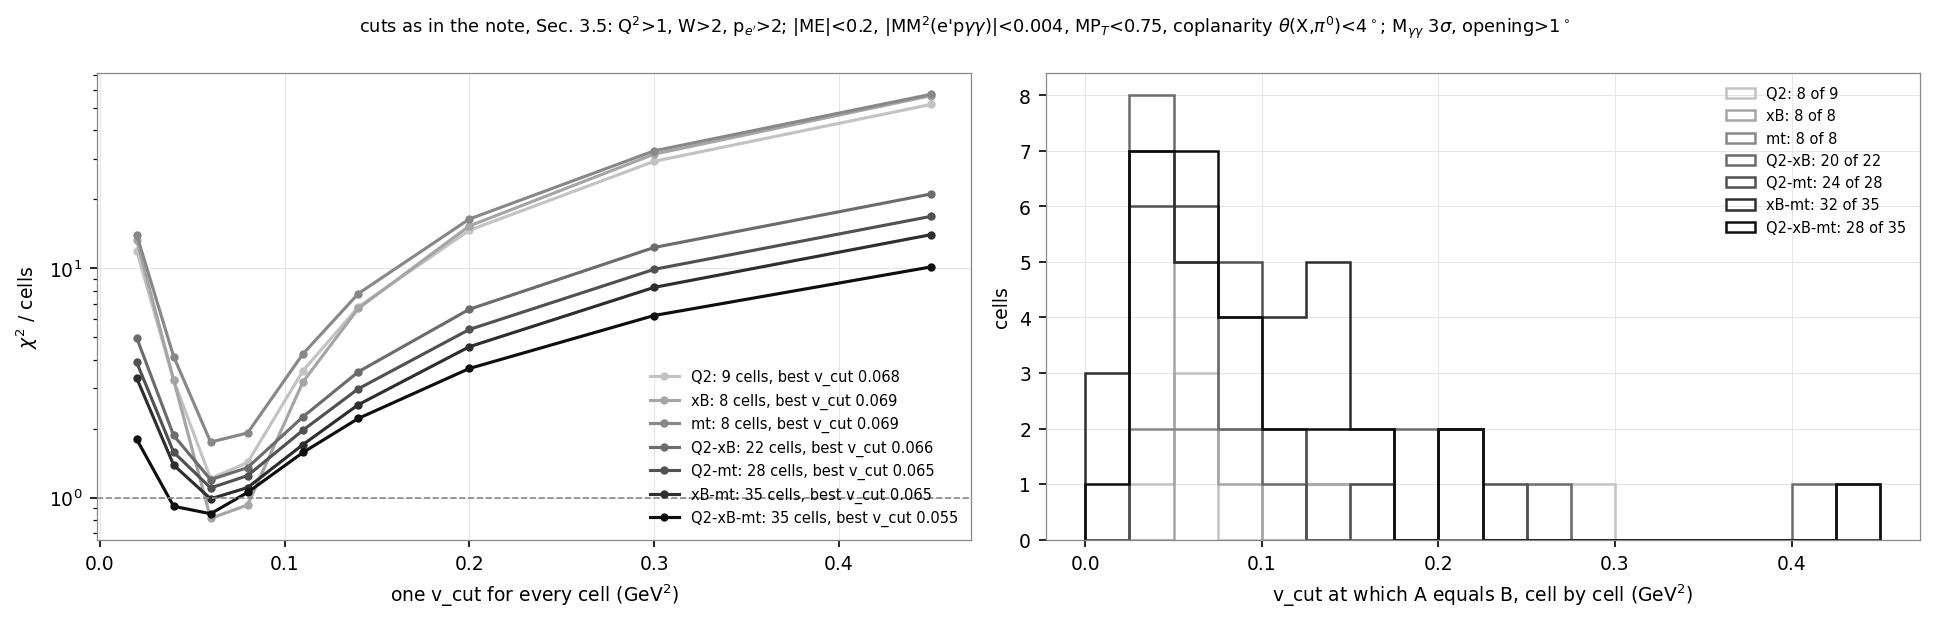
\includegraphics[width=\textwidth]{c4_chi2.png}
\caption{$\chi^2$/cells of one global $\vcut$ for every binning, and the cell-by-cell equivalent
$\vcut$.}
\end{figure}

\begin{table}[H]\centering
\begin{tabular}{lccc}\toprule
binning (rest integrated) & cells & best $\vcut$ & $\chi^2$ at 0.06\\\midrule
$Q^2$ & 9 & 0.068 & 11\\
$x_B$ & 8 & 0.069 & 6\\
$-t$ & 8 & 0.069 & 14\\
$Q^2\times x_B$ & 22 & 0.066 & 26\\
$Q^2\times(-t)$ & 28 & 0.065 & 31\\
$x_B\times(-t)$ & 35 & 0.065 & 35\\
$Q^2\times x_B\times(-t)$ & 35 & 0.055 & 30\\\bottomrule
\end{tabular}
\caption{$\phi$-integrated: one $\vcut\approx0.06$--$0.07$ fits every combination with
$\chi^2/{\rm ndf}\approx1$ at the present 2--10\% errors.}
\end{table}

%=====================================================================
\section{$\phi$ dependence and the structure functions}
\label{sec:phifit}
The final goal is the separation
$d\sigma/d\phi\propto\sigma_U+\varepsilon\sigma_{TT}\cos2\phi+\sqrt{2\varepsilon(1+\varepsilon)}\,\sigma_{LT}\cos\phi$,
$\sigma_U=\sigma_T+\varepsilon\sigma_L$, so the test that matters is not the integral of $\delta$ but
what each correction does to the three structure functions. In two wide bins:

\begin{itemize}
\item pseudo-data: the reconstructed rad MC after the note's cuts, \emph{even} event numbers;
\item $\delta_B$ from the \emph{odd} rad events and the Born MC (so B is not the data divided by itself);
\item $\delta_A$ from \texttt{rc\_factor} per event, $\vcut=0.06$ and $0.2$;
\item $\sigma(\phi)=N_{\rm data}(\phi)/({\rm Acc}_{\rm Born}(\phi)\,\delta(\phi))$, with
  ${\rm Acc}_{\rm Born}$ = Born reconstructed / Born generated in the bin;
\item fitted for $\sigma_U$, $\sigma_{TT}$, $\sigma_{LT}$ with bin-averaged cosines, and compared with
  the same fit of the generated Born distribution (the model).
\end{itemize}

\begin{figure}[H]\centering
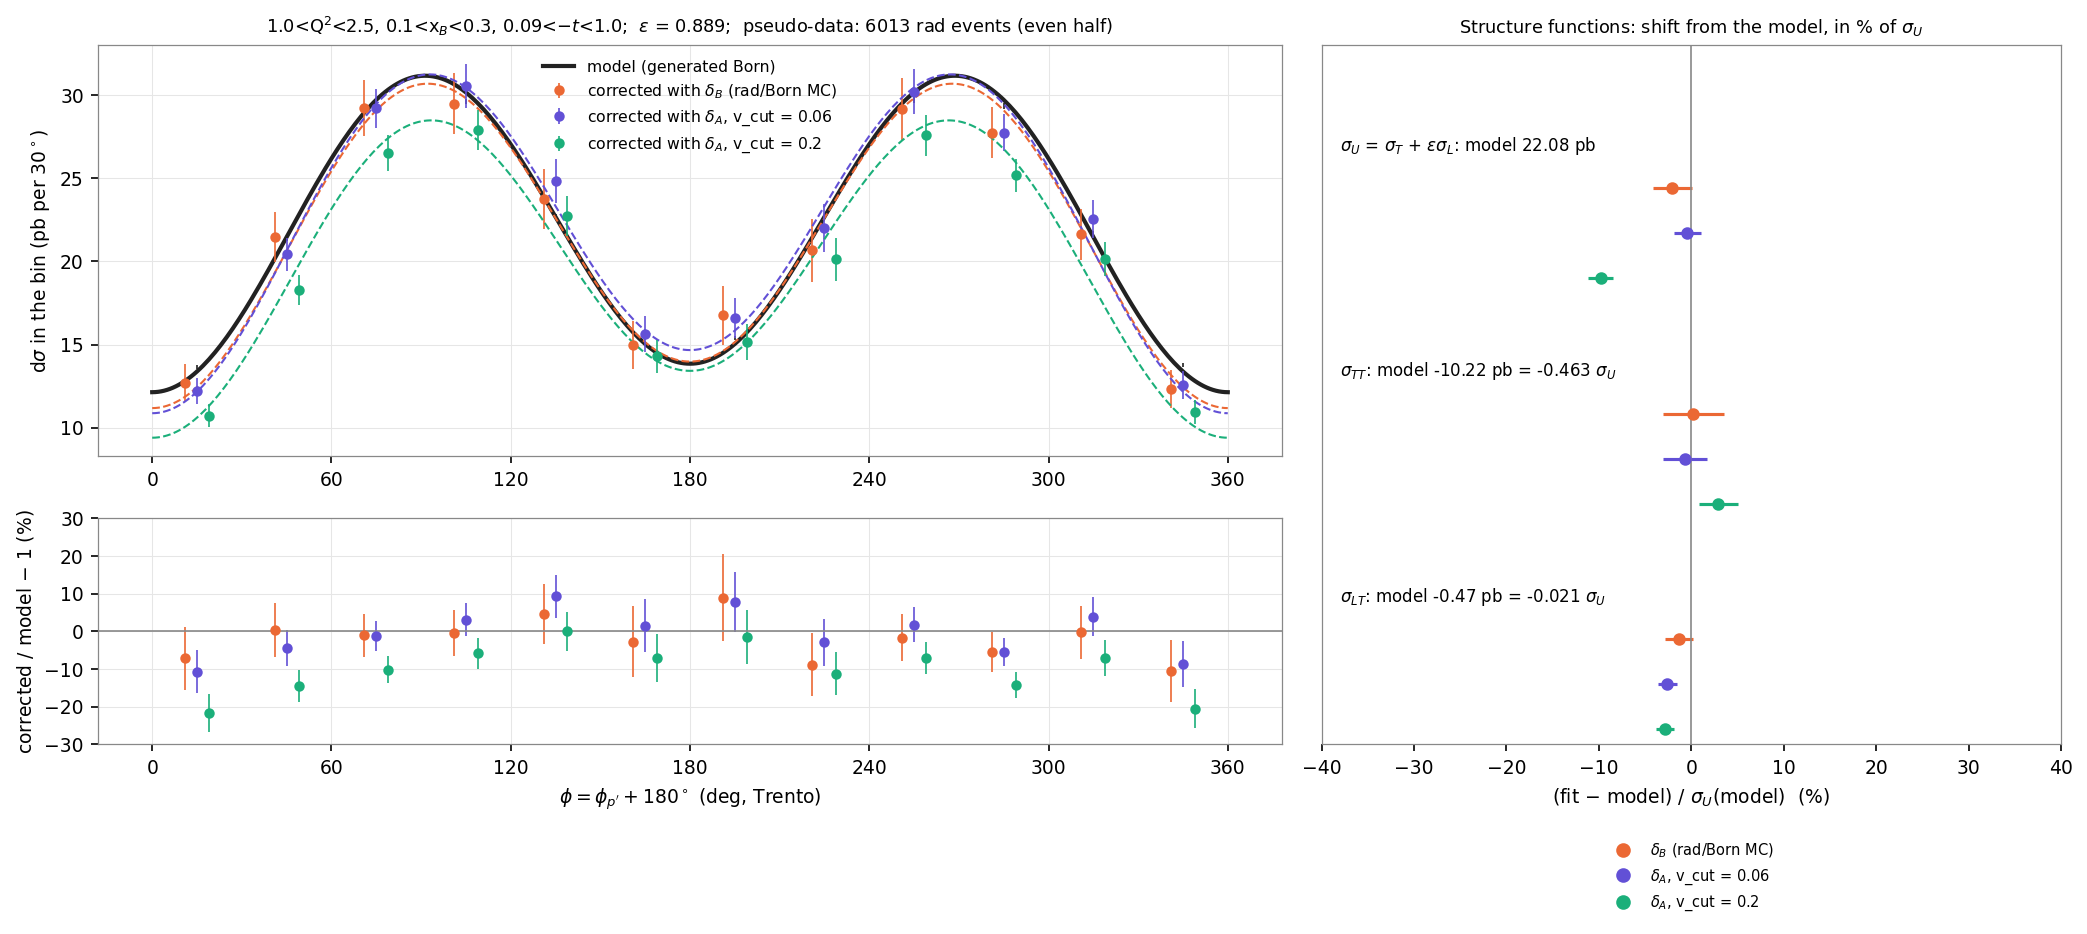
\includegraphics[width=\textwidth]{f_wide2.png}
\caption{Bin $1.0<Q^2<2.5$, $0.10<x_B<0.30$, $0.09<-t<1.0$, $\varepsilon=0.889$, 6013 pseudo-data
events. Left: corrected $\phi$ distributions and fits against the model; corrected/model$-1$ in \%
below. Right: shift of each structure function from the model, in \% of $\sigma_U$.}
\end{figure}
\begin{figure}[H]\centering
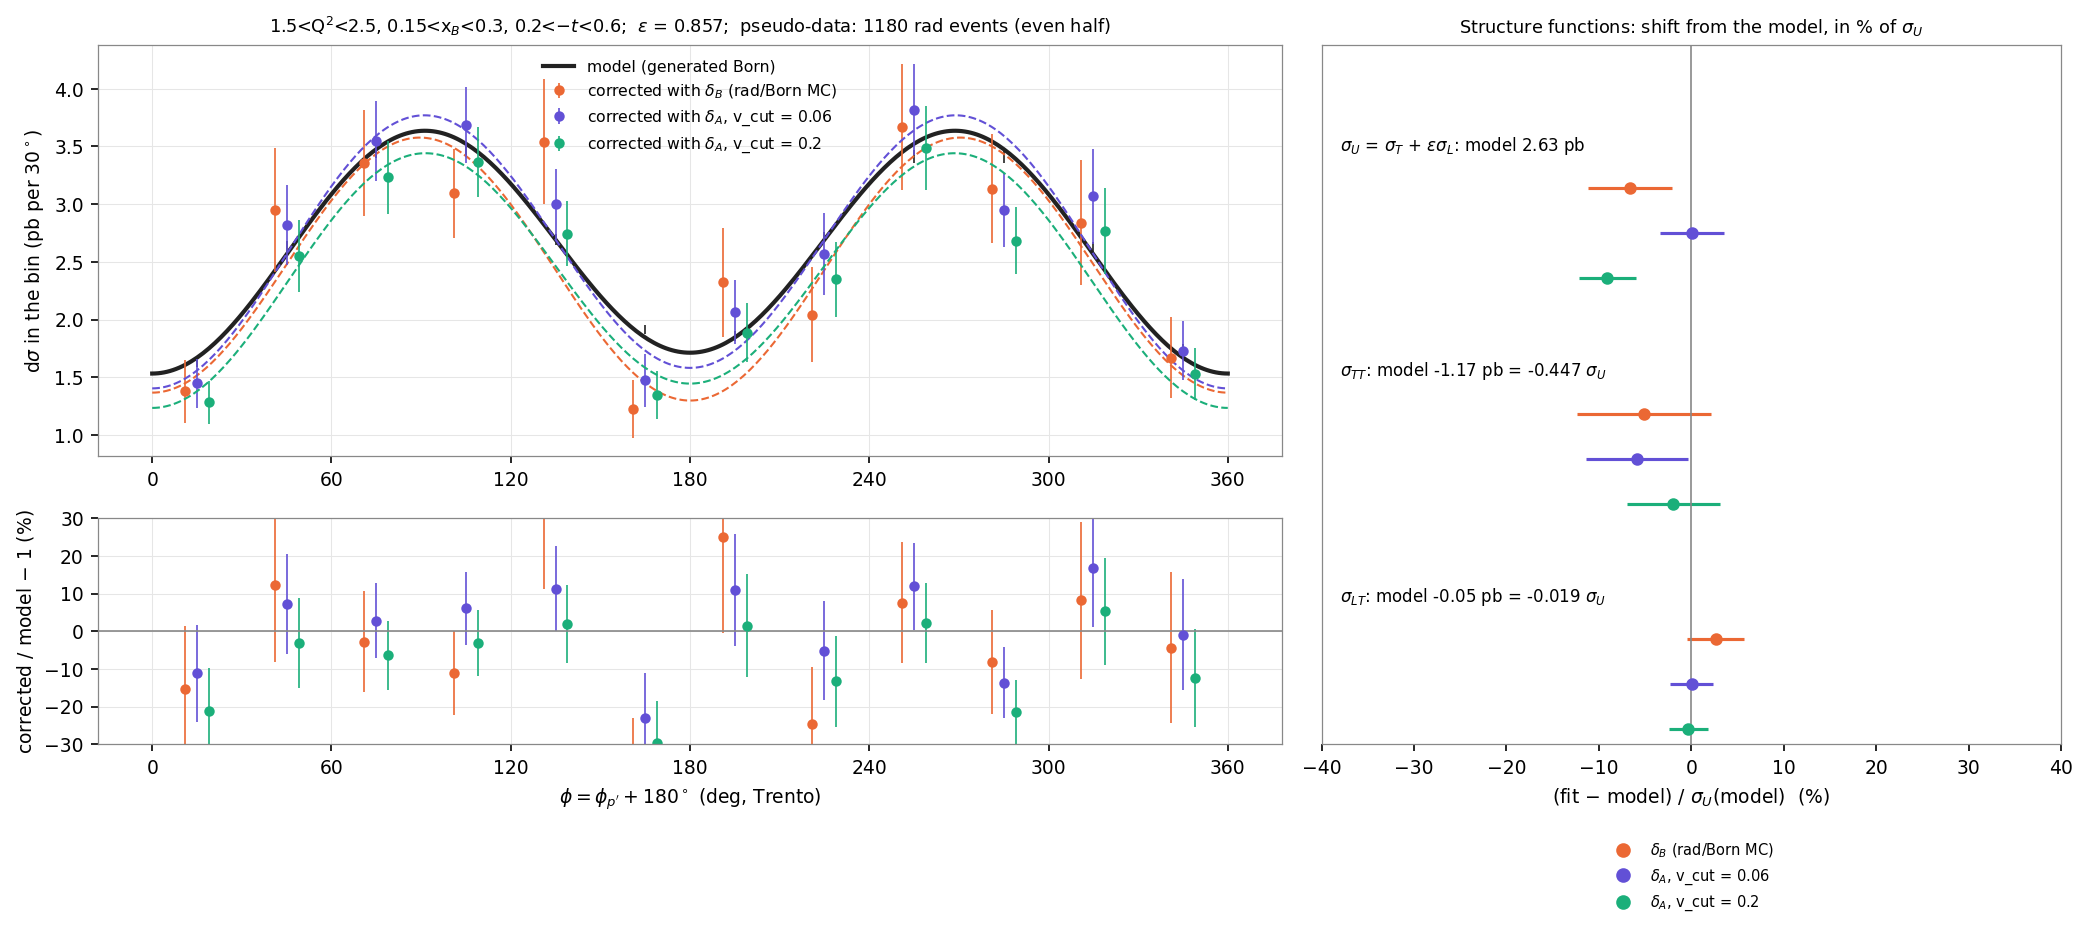
\includegraphics[width=\textwidth]{f_wide1.png}
\caption{Bin $1.5<Q^2<2.5$, $0.15<x_B<0.30$, $0.2<-t<0.6$, $\varepsilon=0.857$: only 1180
pseudo-data events.}
\end{figure}

\begin{table}[H]\centering
\begin{tabular}{llccc}\toprule
bin & correction & $\sigma_U/\sigma_U^{\rm model}$ & $(\sigma_{TT}-\sigma_{TT}^{\rm model})/\sigma_U$ &
$(\sigma_{LT}-\sigma_{LT}^{\rm model})/\sigma_U$\\\midrule
wide2 & B (rad/Born) & $0.979\pm0.021$ & $+0.002\pm0.033$ & $-0.013\pm0.015$\\
(6013 ev.) & A, $\vcut=0.06$ & $0.996\pm0.015$ & $-0.007\pm0.024$ & $-0.026\pm0.011$\\
 & A, $\vcut=0.2$ & $0.902\pm0.014$ & $+0.029\pm0.021$ & $-0.029\pm0.010$\\\midrule
wide1 & B & $0.934\pm0.046$ & $-0.051\pm0.073$ & $+0.027\pm0.031$\\
(1180 ev.) & A, $\vcut=0.06$ & $1.001\pm0.034$ & $-0.059\pm0.055$ & $+0.000\pm0.024$\\
 & A, $\vcut=0.2$ & $0.909\pm0.031$ & $-0.019\pm0.050$ & $-0.003\pm0.021$\\\bottomrule
\end{tabular}
\caption{Model values: wide2 $\sigma_{TT}/\sigma_U=-0.463$, $\sigma_{LT}/\sigma_U=-0.021$;
wide1 $-0.447$ and $-0.019$.}
\end{table}

What this shows, at this statistics:
\begin{itemize}
\item $\vcut=0.2$ underestimates $\sigma_U$ by 10\% ($7\sigma$ in wide2); $\vcut=0.06$ and B recover it.
\item The errors on $\sigma_{TT}$ are 2--3\% of $\sigma_U$ (5--7\% of $\sigma_{TT}$) in the larger bin,
  5--7\% of $\sigma_U$ in the smaller. Differences between the corrections are within them.
\item $\sigma_{LT}$ is small here ($\approx-0.02\,\sigma_U$) and its error, 0.010--0.015\,$\sigma_U$, is
  as large as $\sigma_{LT}$ itself. The A-corrected $\sigma_{LT}$ sits $0.026\pm0.011\,\sigma_U$
  below the model ($2.4\sigma$), B $0.013\pm0.015$: suggestive, not conclusive.
\item The data error dominates; the B correction adds its own statistical error, which A does not.
\end{itemize}
\textbf{The $\phi$ dependence of the correction, and with it the effect on $\sigma_{TT}$ and
$\sigma_{LT}$, cannot be settled with the present sample.}

%=====================================================================
\section{Conclusions so far}

\begin{enumerate}
\item \textbf{The engine is consistent with itself.} At generator level, with the same $\mmep$ cut,
  A and B agree in shape; the residual $+3\%$ is \texttt{itarg} in the Born arm.
\item \textbf{$\phi$ must be defined as in EXCLURAD}, $\phi_{p'}+180^\circ$, in the analysis and in
  the RC alike.
\item \textbf{Only $ME$ and $\mmtot$ cut radiation}; $MP_T$ and coplanarity add nothing once they are
  applied. Together they act as a soft cut on the true $v$ with its 50\% point at $v=0.057$.
\item \textbf{$\phi$-integrated}, one $\vcut\approx0.06$--$0.07~\mathrm{GeV^2}$ reproduces B in every
  combination of $Q^2$, $x_B$, $-t$ within 2--10\%; $\vcut=0.2$ is 5--10\% off. The equivalent $\vcut$
  is a property of the exclusivity windows and the resolution (0.14 with wider windows), and must be
  derived for each cut chain.
\item \textbf{No definite conclusion is possible yet on the $\phi$ dependence.} An integrated agreement
  says nothing about the $\cos\phi$ and $\cos2\phi$ terms of $\delta$. A difference
  $\delta_B/\delta_A=1+a\cos\phi+b\cos2\phi$ shifts $\sigma_{LT}$ by $\approx a\,\sigma_U/\sqrt{2\varepsilon(1+\varepsilon)}$
  and $\sigma_{TT}$ by $\approx b\,\sigma_U/\varepsilon$; for $\pi^0$, where $\sigma_{TT}$ and
  $\sigma_{LT}$ are a fraction of $\sigma_U$, a 2--3\% term becomes a 10--30\% change of the
  structure function. The separation of $\sigma_T+\varepsilon\sigma_L$, $\sigma_{TT}$, $\sigma_{LT}$
  is the goal of the experiment, so this is the test that matters, and the present statistics cannot
  make it.
\end{enumerate}

\section{What is needed}
\begin{itemize}
\item \textbf{Statistics}: $\sim10^4$ accepted events per arm per bin to measure the $\cos\phi$ and
  $\cos2\phi$ terms of $\delta$ to $\approx1\%$; roughly 10--20M generated per arm and polarity for a
  few wide bins, more for the note's grid.
\item Born arm with \texttt{itarg}=0.
\item Pseudo-data from a \emph{different} model (\texttt{amp2614}) than the correction
  (\texttt{amp2609} twins), so the test is not circular.
\item Vertex and sector in the ntuple, to apply the note's vertex and same-sector cuts.
\item The comparison made on the extracted $\sigma_U$, $\sigma_{TT}$, $\sigma_{LT}$, as in
  Sec.~\ref{sec:phifit}.
\end{itemize}

\appendix
\section{Reproducibility}
Branch \texttt{rc-method-comparison} of \texttt{github.com/vkubarovsky/exclurad\_py}, directory
\texttt{docs/rc\_method\_pi0/}; scripts \texttt{production/analysis/rc\_method\_pi0*.py}.
Ntuples and per-event $\eta$ tables: \texttt{/Volumes/wd\_14tb/rc\_method\_pi0/}.

\end{document}
